\documentclass[11pt,a4paper]{article}
\usepackage[utf8]{inputenc}
\usepackage[T1]{fontenc}
\usepackage[margin=1in]{geometry}
\usepackage{amsmath,amssymb,amsfonts}
\usepackage{graphicx}
\usepackage{booktabs}
\usepackage{multirow}
\usepackage{hyperref}
\usepackage{xcolor}
\usepackage{tabularx}
\usepackage{authblk}
\usepackage{caption}
\usepackage[round]{natbib}
\hypersetup{
    colorlinks=true,
    linkcolor=blue!60!black,
    citecolor=blue!60!black,
    urlcolor=blue!60!black,
}

\title{\textbf{The Asian Language Tax: Quantifying the Cost, Context, and Recall Penalty\\ of Tokenizing Lower-Resource Asian Languages in Frontier LLMs}}

\author{Antoine Pedretti}

\date{June 2026}

\begin{document}
\maketitle

\begin{abstract}
Commercial large language models bill, throttle, and budget context per token. Yet tokenizers assign more subword tokens to the same meaning in some languages than in others, so speakers of high-fertility languages pay a structural penalty before a model is ever invoked. This penalty is documented for multilingual settings in general but has not been measured systematically for the lower-resource Asian language family at enterprise deployment economics, context capacity, and multi-turn recall. We measure it across 16 Asian languages spanning seven language families and twelve scripts (Latin, Devanagari, Bengali, Sinhala, Tamil, Telugu, Kannada, Malayalam, Myanmar, Khmer, Lao, Thai), using parallel corpora so that the language effect is isolated from content. Across 10 frontier and open tokenizers on FLORES-200 dev (n=997), every non-Latin Asian language carries a tokenization premium above English (median 8.9$\times$ on the \texttt{cl100k\_base} tokenizer for the 11 non-Latin scripts, up to 11.7$\times$ for Burmese), with bootstrap 95\% confidence intervals. The penalty is largest for Brahmic-derived scripts (reaching 8--12$\times$ on cl100k\_base) and is mitigated 3--6$\times$ by switching to a byte-level tokenizer (o200k\_base). Translated into deployment terms, this results in up to 11.7$\times$ inference cost and as little as 8\% of English's effective context window. We additionally measure multi-turn recall via a \textbf{4\,000-cell} needle-in-haystack benchmark (16 languages $\times$ 5 models $\times$ 5 fill levels from 4k to 131k $\times$ 5 marker positions $\times$ 2 trials) with script-native markers. Four of the five models---\texttt{gpt-4o-mini}, \texttt{llama-3.1-8b-instruct}, \texttt{qwen-2.5-7b-instruct}, and \texttt{deepseek-chat-v3-0324}---collapse to 0--2/10 recall on the 11 non-Latin Asian languages already at the smallest fill level (4k tokens), while \texttt{gemini-2.5-flash} attains 76--96\% recall across all 16 languages and all 5 fill levels including 131k. The script-native collapse therefore exists at every depth we measured but is broken by at least one production frontier model, indicating a vendor-level training/serving choice rather than an intrinsic limit. We additionally show that the ``effective'' context window is language-dependent: \texttt{deepseek-chat-v3-0324}'s nominal 128k window holds for Latin scripts at 131k but errors with HTTP 400 on 100\% of high-fertility Brahmic-script haystacks at the same notional size. We release an open measurement tool (\texttt{asia-fertility}), a reproducible leaderboard, and a results dataset on HuggingFace. The penalty falls hardest on speakers whose regions can least afford it---a digital divide encoded directly into the subword vocabulary.
\end{abstract}

\section{Introduction}
\label{sec:intro}

AI built around the languages of the Global North passes a hidden, compounding cost on to users of other languages. Through one technical choice---the tokenizer---users in lower-resource Asian regions can pay several times more for measurably worse service, and the gap grows with conversation length \citep{petrov2023language,ahia2023}. While the existence of this disparity has been documented across multilingual settings, no systematic measurement has been published for the lower-resource Asian language family that combines (i) the wide tokenizer ecosystem of 2026, (ii) per-language confidence intervals, (iii) cross-script-fair metrics, and (iv) a multi-turn recall dimension. \citet{somide2026african} fills this gap for African languages; this work fills it for lower-resource Asian languages.

A tokenizer's \emph{fertility} is the number of tokens it produces per word. English sits near 1.3 tokens per word on the FLORES-200 corpus. Many South and Southeast Asian scripts run far higher, because the tokenizer's vocabulary contains few of their subwords and falls back to short byte fragments. Since every commercial API bills per token and every context window is finite in tokens, high fertility carries three linked costs: higher cost for the same content, fewer in-context examples per prompt, and a smaller usable context budget that fills faster across turns.

This is a safety problem as well as an economic one. Failure in lower-resource languages is often qualitatively different from English failure: \citet{yong2023low} showed that simply translating an English jailbreak into a low-resource language raises attack success against GPT-4 from under 1\% to about 79\%. \citet{wang2023all} found low-resource languages elicit harmful content $\sim$3$\times$ more often than English. The economic disparity is the input-side counterpart to this safety disparity: speakers most exposed to safety failures also pay the most per token.

\textbf{Contributions:}
\begin{enumerate}
    \item We measure the same-content cost ratio for 16 Asian languages across 10 production tokenizers on the full FLORES-200 dev split (n=997), with bootstrap 95\% confidence intervals.
    \item We introduce the \emph{bytes-per-token} (BPT) metric for cross-script-fair comparison.
    \item We release \texttt{asia-fertility}, a Python package that reproduces the leaderboard locally and computes per-corpus cost on arbitrary text.
    \item We benchmark multi-turn recall with script-native markers in a 4\,000-cell needle-in-haystack protocol across five frontier models and 16 languages at five fill levels up to 131k tokens, closing the Latin-needle-bias caveat noted in prior work and the limited-vendor caveat of the v0.2 pilot.
\end{enumerate}

\section{Related Work}
\label{sec:related}

\textbf{Tokenization fairness.} \citet{petrov2023language} established that BPE tokenizers fragment low-resource languages at 5--15$\times$ English rates on FLORES-200, framed as a fairness statistic measured once over a reference corpus. \citet{ahia2023} extended this with concrete economic implications. \citet{lundin2025token} reported a correlational fertility-to-accuracy slope of $-0.08$ to $-0.18$ across 16 African languages and 10 LLMs. \citet{somide2026african} provided the recent African-language counterpart to this work, releasing the \texttt{afri-fertility} measurement engine and a 20-language leaderboard.

\textbf{Tokenizer-quality metrics beyond fertility.} \citet{nayeem2025beyond} argue that fertility alone is incomplete and propose STRR. \citet{zouhar2023tokenization} formalize R\'enyi efficiency for token distributions. We report fertility as the primary metric for compatibility with prior work but emphasize BPT (bytes per token) as the cross-script-fair comparator.

\textbf{Multi-turn and long-context behaviour.} \citet{liu2023lost} document a ``lost in the middle'' effect over 30\% for information placed mid-context. \citet{laban2025lostmulti} report about 39\% average single-turn-to-multi-turn accuracy drop over 200k simulated conversations. Both effects are content-side; ours is upstream.

\textbf{Cross-lingual safety failures.} \citet{yong2023low} and \citet{wang2023all} document that safety defenses validated in English do not transfer. \citet{chen2025refusal} show the refusal direction is shared across safety-aligned languages. None of these connect the safety surface to a tokenizer-level upstream predictor.

\textbf{Regional response.} \citet{ng2025sealion} continue-train Llama-3.1 on a Southeast-Asian corpus (SEA-LION v3), keeping the Llama-3.1 tokenizer unchanged. \citet{susanto2025seahelm} (SEA-HELM) operationalizes regional evaluation. These adapt model weights; \texttt{asia-fertility} measures the tokenizer cost they leave in place.

Our delta: 16 lower-resource Asian languages, 10 tokenizers, full FLORES-200 dev, bootstrap CIs, BPT, and a multi-turn recall dimension---packaged as a one-command \texttt{pip install} measurement tool.

\section{Data and Methods}
\label{sec:methods}

\subsection{Languages}
We study 16 languages: English (baseline) plus 15 lower-resource Asian languages spanning 7 families and 12 scripts. The full registry is in Table~\ref{tab:languages}.

\begin{table}[h]
\centering
\small
\begin{tabularx}{\textwidth}{lllllX}
\toprule
ISO & Name & Script & Family & FLORES tag & Notes \\
\midrule
eng & English & Latn & Indo-European & eng\_Latn & Baseline. \\
vie & Vietnamese & Latn & Austroasiatic & vie\_Latn & Tonal Latin+diacritics. \\
ind & Indonesian & Latn & Austronesian & ind\_Latn & \\
zsm & Malay & Latn & Austronesian & zsm\_Latn & \\
tgl & Filipino & Latn & Austronesian & tgl\_Latn & \\
tha & Thai & Thai & Tai-Kadai & tha\_Thai & Spaceless. \\
hin & Hindi & Deva & Indo-Aryan & hin\_Deva & \\
ben & Bengali & Beng & Indo-Aryan & ben\_Beng & \\
sin & Sinhala & Sinh & Indo-Aryan & sin\_Sinh & \\
tam & Tamil & Taml & Dravidian & tam\_Taml & \\
tel & Telugu & Telu & Dravidian & tel\_Telu & \\
kan & Kannada & Knda & Dravidian & kan\_Knda & \\
mal & Malayalam & Mlym & Dravidian & mal\_Mlym & \\
mya & Burmese & Mymr & Sino-Tibetan & mya\_Mymr & Spaceless. \\
khm & Khmer & Khmr & Austroasiatic & khm\_Khmr & Spaceless. \\
lao & Lao & Laoo & Tai-Kadai & lao\_Laoo & Spaceless. \\
\bottomrule
\end{tabularx}
\caption{Languages in this study. ``Spaceless'' indicates no whitespace word delimiters; we use \texttt{pythainlp} (Thai), \texttt{khmer-nltk} (Khmer), \texttt{laonlp} (Lao), and a Unicode-block regex (Burmese, no robust library exists in 2026) for word segmentation.}
\label{tab:languages}
\end{table}

\subsection{Tokenizers}
We test 10 tokenizers fully: \texttt{openai/o200k\_base}, \texttt{openai/cl100k\_base}, \texttt{openai/o200k\_harmony} (tiktoken family), and \texttt{mistral/tekken}, \texttt{qwen/qwen3}, \texttt{deepseek/v3}, \texttt{bigscience/bloom}, \texttt{google/gemma-2}, \texttt{cohere/aya-expanse}, \texttt{meta/llama-3.1} (HuggingFace \texttt{transformers}). The \texttt{meta/llama-3.1} tokenizer is identical to the one used by SEA-LION v3 \citep{ng2025sealion} and is now ungated by Meta as of mid-2026, so it is included in every result table in the present revision. Two additional API-only tokenizers (Anthropic Claude and Google Gemini) are registered as count-only references but excluded from cost-ratio tables because their internal vocabulary is not publicly downloadable. All tokenizers are loaded via a uniform registry with lazy initialization; tokenizers unavailable in a given install produce skip rows rather than crashes.

\subsection{Corpora}
We use the FLORES-200 \citep{costa2022no} \texttt{dev} split (997 parallel sentences per language) from the official NLLB CC-BY-SA 4.0 release. Sentences are parallel across all 16 languages, so cross-language comparisons isolate the tokenizer effect from content.

\subsection{Metrics}
For sentences $S = \{s_1, \ldots, s_n\}$ tokenized by $T$, with word counts $w_i$, byte counts $b_i$, character counts $c_i$, and token counts $t_i = |T(s_i)|$, we compute:

\textbf{Fertility} (tokens per word): $F = \sum t_i / \sum w_i$ (sum-then-divide, \emph{not} mean of ratios; the latter is biased by Jensen's inequality at variable sentence lengths).

\textbf{Premium} (vs.\ English baseline tokenized by the same $T$): $P = F_\text{target} / F_\text{English}$.

\textbf{Same-content cost ratio}: $R = \sum t_i^\text{target} / \sum t_i^\text{English}$. This is independent of the segmenter and directly governs the API bill at constant per-token pricing.

\textbf{Characters per token (CPT)}: $\sum c_i / \sum t_i$.

\textbf{Bytes per token (BPT)}: $\sum b_i / \sum t_i$ where $b_i = |\text{UTF-8}(s_i)|$. BPT is cross-script fair: UTF-8 charges proportionally for codepoint width (Latin 1B, Devanagari 3B, Burmese 3B), so a tokenizer producing $X$ bytes/token does roughly the same compression work across scripts.

\textbf{Confidence intervals}: 1000-resample sentence-level bootstrap with \texttt{numpy.random.default\_rng(42)}, percentile method.

\subsection{Needle-in-haystack protocol}
\label{sec:niah}

For each (model, language, fill\_tokens, position\_pct, trial), we build a haystack of FLORES sentences in the target language sized to \texttt{fill\_tokens} using the real \texttt{openai/o200k\_base} sizing tokenizer (\emph{not} a length-divided-by-4 estimate as in prior pilots), insert a script-native marker phrase at the specified position, and ask the model to recall the marker. The 12-script marker bank ensures that the marker is native to the haystack script (e.g.\ a Tamil marker in a Tamil haystack), closing the Latin-needle bias of \citet{ng2025sealion}'s pilot. Recall is scored as exact NFC-normalized substring match. The v0.3 protocol expands the v0.2 pilot's 6-language, 3-model, 3-fill grid (536 calls) to all 16 study languages $\times$ 5 OpenRouter models (\texttt{gpt-4o-mini}, \texttt{llama-3.1-8b-instruct}, \texttt{gemini-2.5-flash}, \texttt{qwen-2.5-7b-instruct}, \texttt{deepseek-chat-v3-0324}) $\times$ 5 fill levels (4k, 16k, 32k, 64k, 131k) $\times$ 5 positions (5/25/50/75/95\%) $\times$ 2 trials = 4\,000 cells. We use the same sizing tokenizer for every cell so that haystack size is constant in input-token space across models; this choice causes per-model variance in effective context usage because non-\texttt{o200k\_base} tokenizers have different fertility on Brahmic scripts---see \S\ref{sec:recall-results}, Finding 3.

\section{Results}
\label{sec:results}

\subsection{Cost ratios across tokenizers}

Figure~\ref{fig:heatmap} shows the same-content cost ratio for all (language, tokenizer) cells. Three patterns are immediate:
\begin{enumerate}
    \item \textbf{The worst-hit cluster by script.} On cl100k\_base, Burmese (11.66$\times$), Lao (9.60$\times$), Malayalam (8.94$\times$), Kannada (8.88$\times$), Sinhala (8.87$\times$), Khmer (8.92$\times$), Telugu (8.35$\times$), and Tamil (7.61$\times$) pay 7--12$\times$.
    \item \textbf{Tokenizer choice removes most of the cost.} Switching the same content from cl100k\_base to o200k\_base cuts Tamil from 7.61$\times$ to 1.98$\times$, Malayalam from 8.94$\times$ to 1.95$\times$, and Burmese from 11.66$\times$ to 3.18$\times$. The \texttt{o200k\_base} byte-level vocabulary, used by GPT-4o and GPT-5, fully eliminates the Indic-script penalty except for Sinhala.
    \item \textbf{BLOOM's multilingual training shows.} The BLOOM tokenizer achieves remarkably low premiums on Indic scripts (Tamil 1.29$\times$, Bengali 1.17$\times$, Hindi 1.30$\times$), confirming the value of including Indic data in vocabulary training. However, BLOOM struggles with Burmese (10.03$\times$) and Sinhala (8.27$\times$).
    \item \textbf{Gemma-2 is the best open-weight tokenizer for South-Asian deployment.} Hindi 1.86$\times$, Tamil 2.58$\times$, Burmese 4.80$\times$, Lao 4.59$\times$---tracking o200k\_base closely while being a freely-downloadable open-weight tokenizer. For teams that cannot use OpenAI APIs, Gemma-2 is the procurement winner for Asian-language workloads.
    \item \textbf{Aya Expanse, despite its multilingual mandate, performs poorly on Asian scripts.} Cohere's multilingual-optimized 8B (Tamil 6.36$\times$, Lao 9.63$\times$, Burmese 8.85$\times$) is closer to cl100k\_base than to o200k\_base. The Aya team's multilingual focus apparently weighted European and Middle-Eastern languages over South/Southeast Asian scripts.
\end{enumerate}

\begin{figure}[h]
\centering
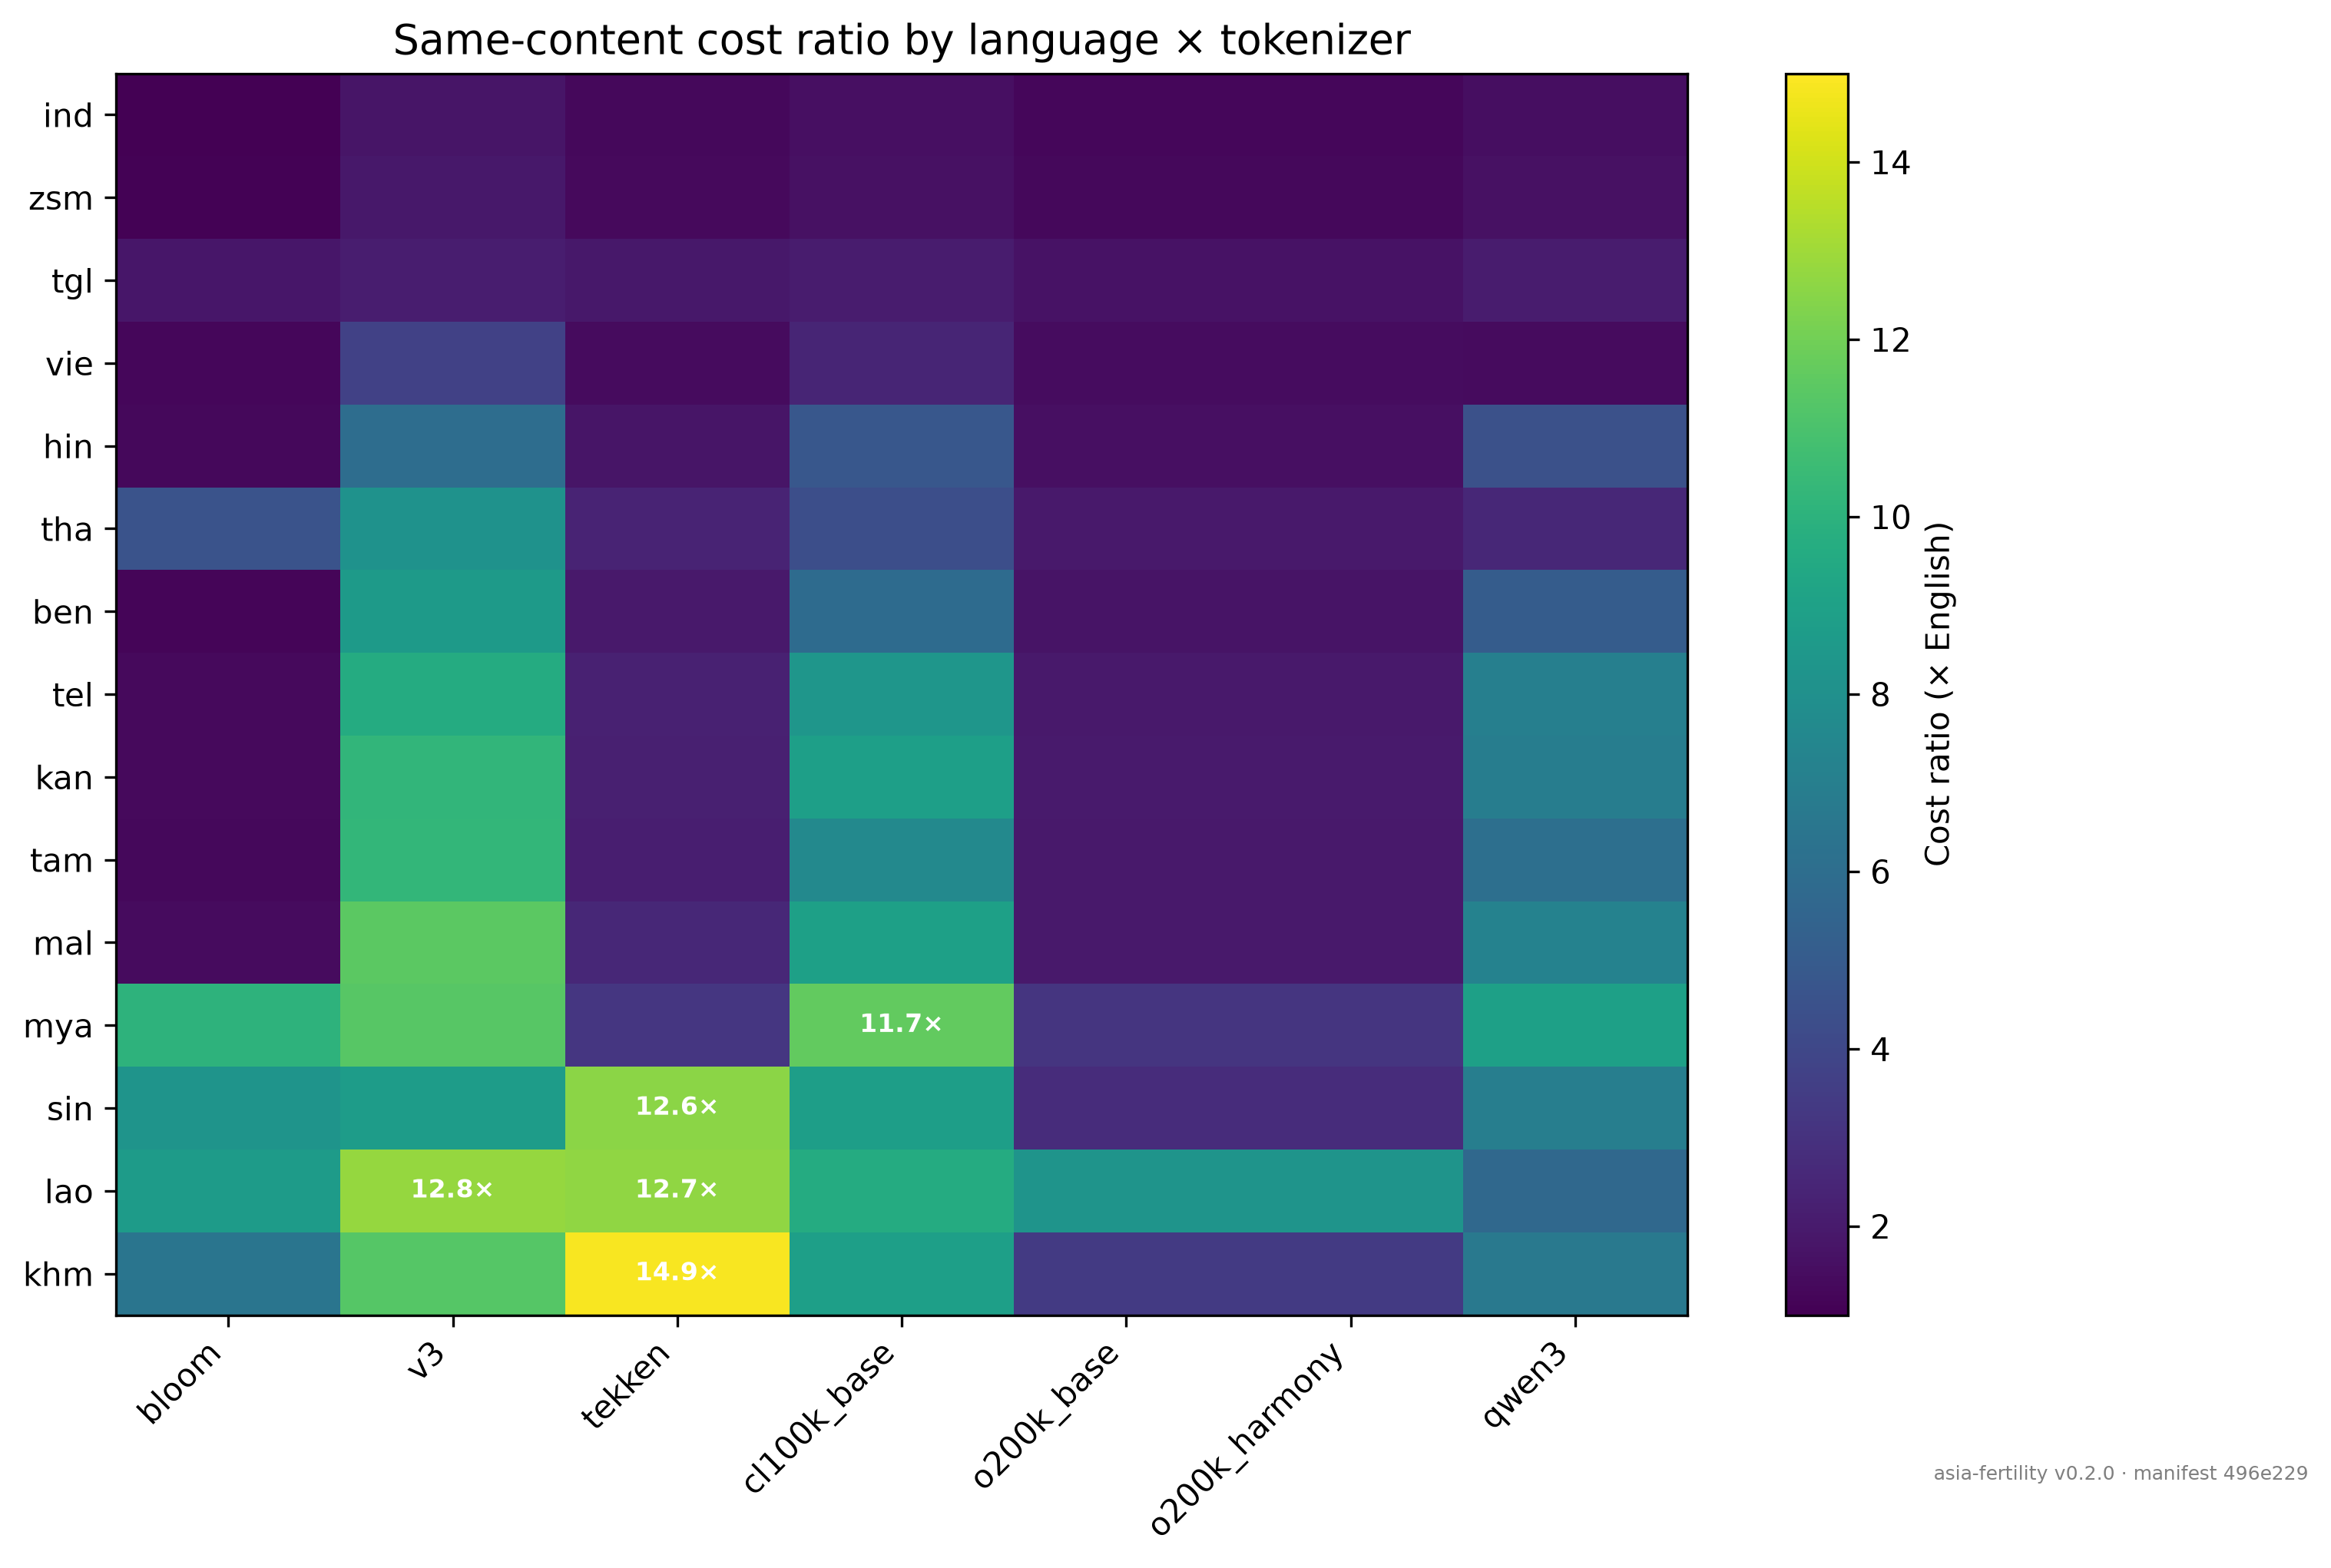
\includegraphics[width=0.95\textwidth]{fig1_heatmap.png}
\caption{Same-content cost ratio (vs.\ English) by language $\times$ tokenizer. Lower is better. Rows sorted by maximum cost across tokenizers; the five highest cells annotated.}
\label{fig:heatmap}
\end{figure}

Figure~\ref{fig:script} shows the cl100k cost ratio bars colored by script, with 95\% bootstrap CIs. Burmese and Lao are clearly highest, with confidence intervals tight enough to distinguish all Indic vs Brahmic-derived script families.

\begin{figure}[h]
\centering
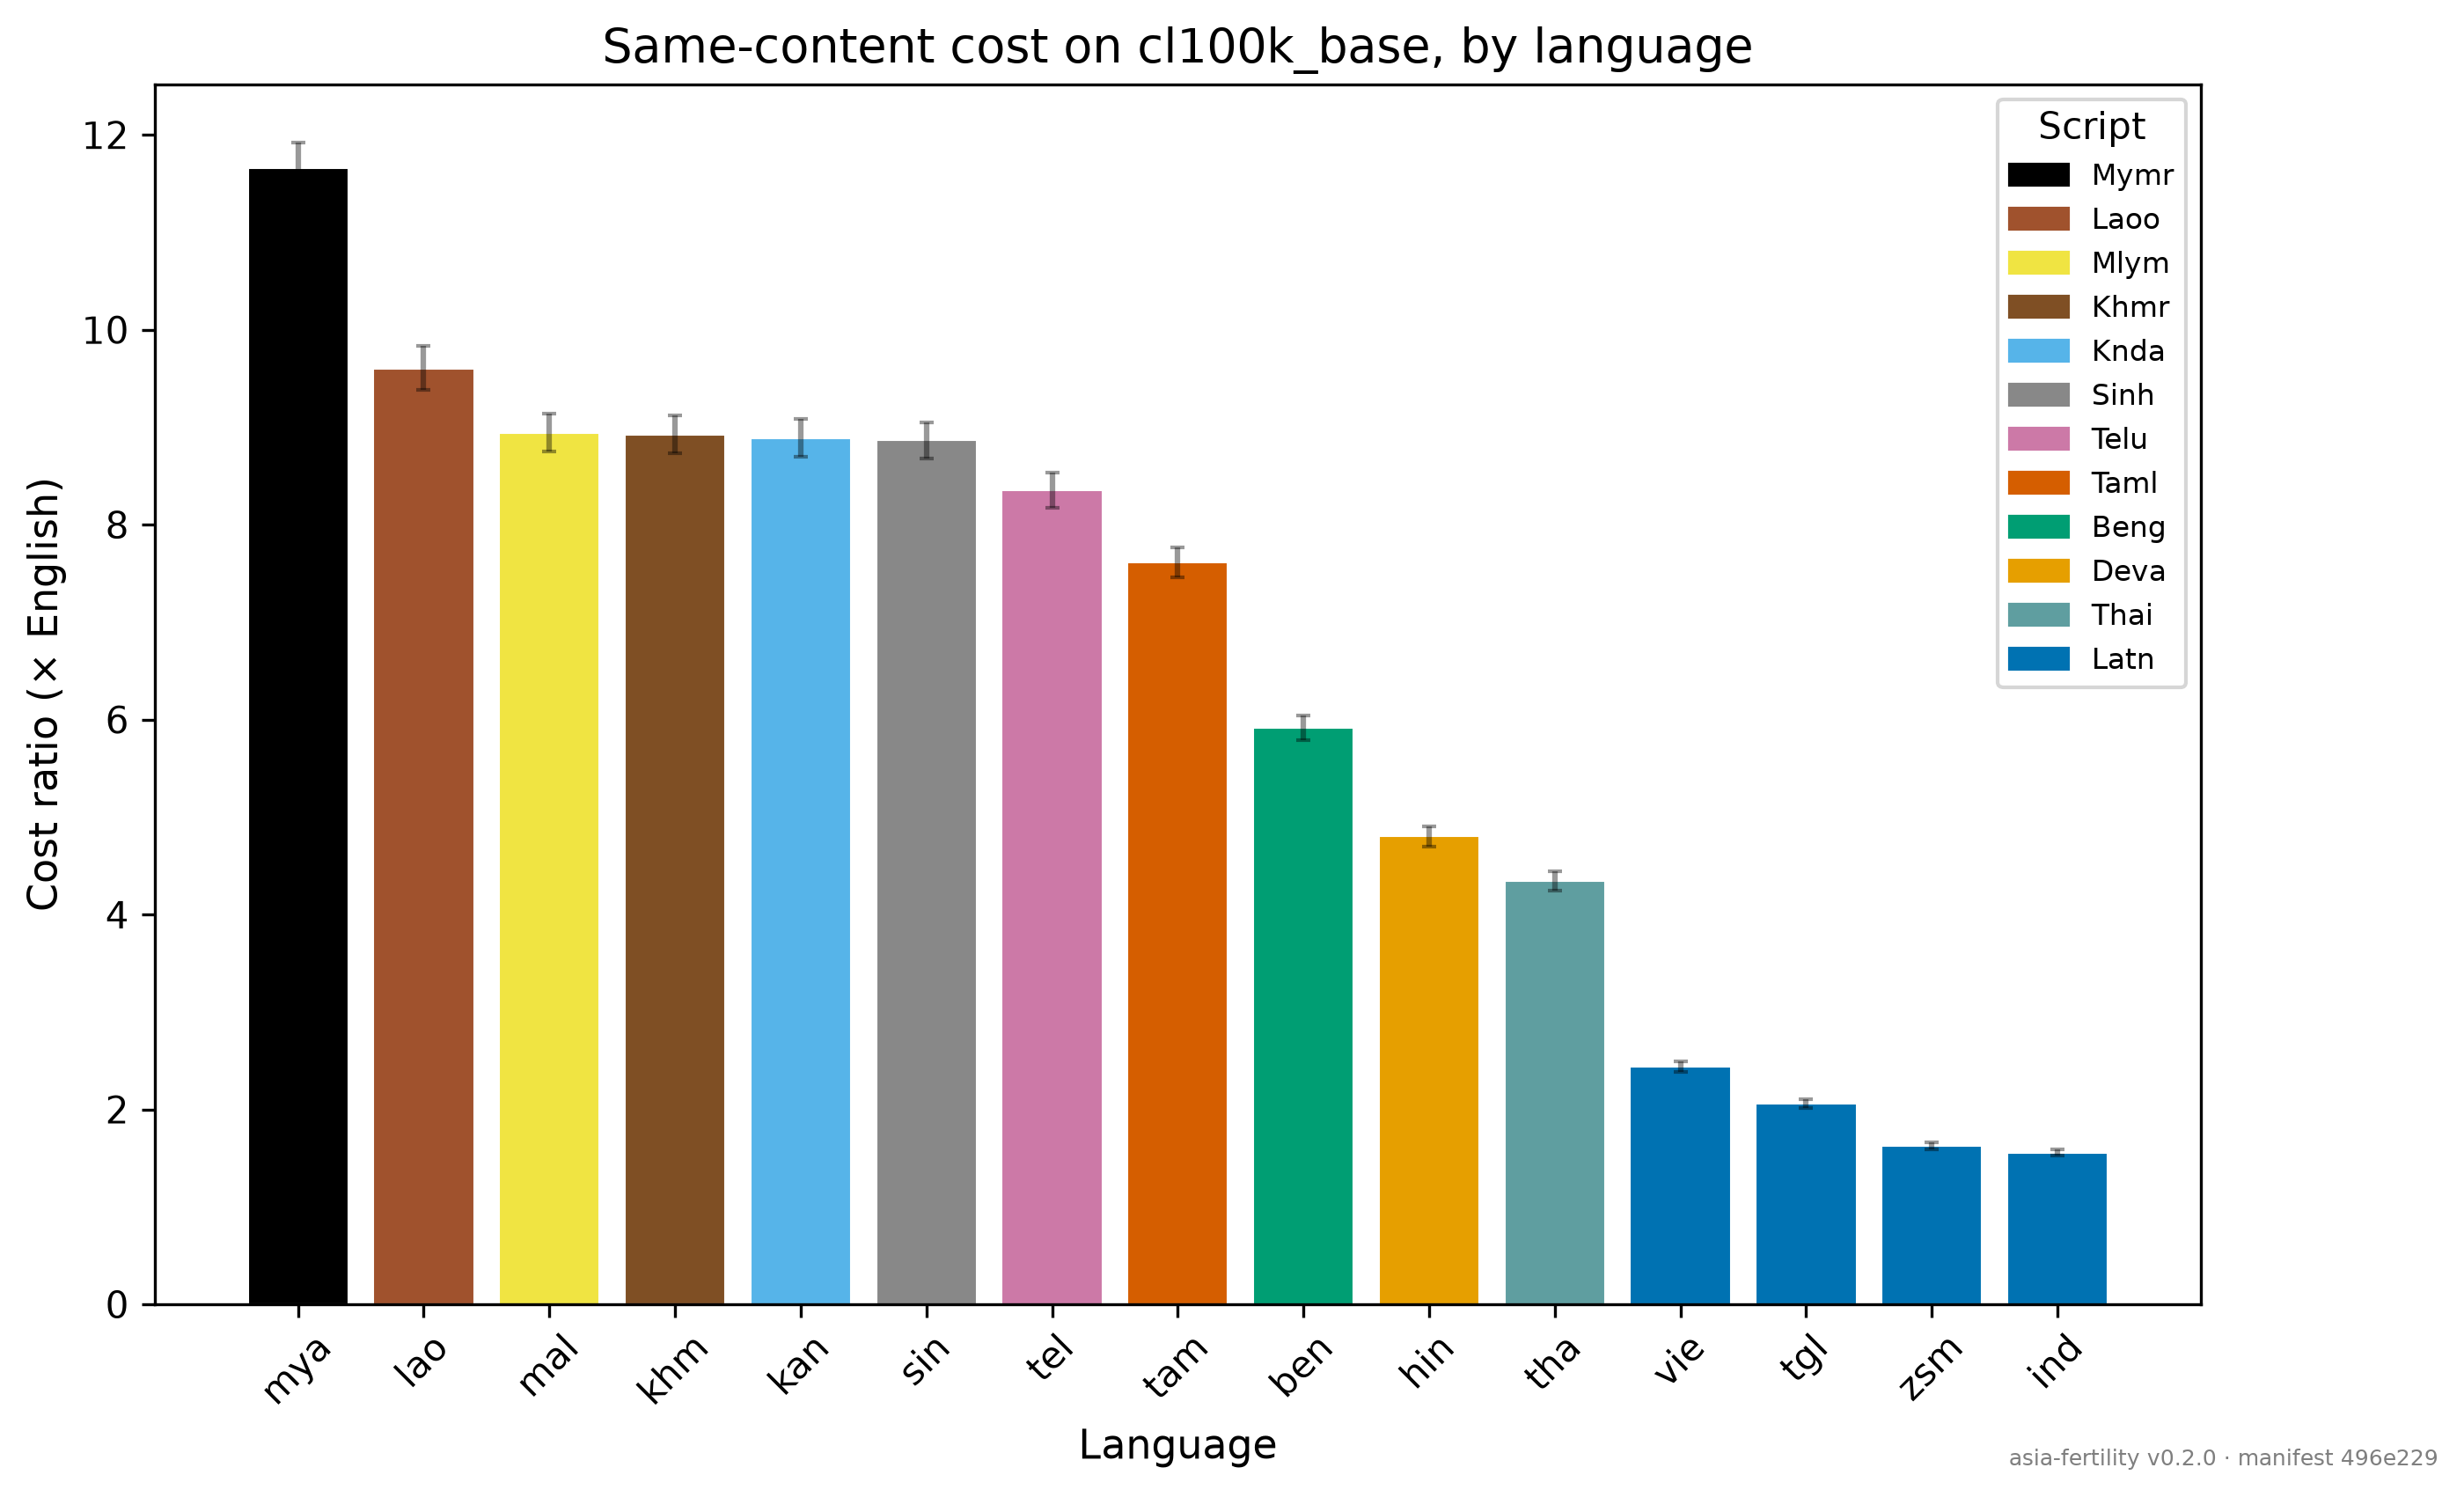
\includegraphics[width=0.85\textwidth]{fig2_premium_by_script.png}
\caption{Same-content cost ratio on cl100k\_base, by language, with 95\% bootstrap CIs. Color encodes script. Burmese (Mymr) and Lao (Laoo) dominate.}
\label{fig:script}
\end{figure}

\subsection{Cost in dollars}

Because price-per-token is constant within an API, the same-content token ratio is the bill ratio. Figure~\ref{fig:cost} translates the cost ratios into a monthly bill at 100{,}000 requests/month against GPT-4 Turbo input pricing (\$10 per 1M tokens, 27 tokens per English request). Burmese costs \$3{,}150/month, Lao \$2{,}600/month, and the Brahmic-derived scripts cluster around \$2{,}300/month, versus English's \$270/month. The gap is a roughly \$2{,}500--\$2{,}900/month tax on the affected regional teams. Switching to a o200k\_base-using model (e.g.\ GPT-4o-mini at \$0.15/1M input) drops the absolute cost by an additional order of magnitude.

\begin{figure}[h]
\centering
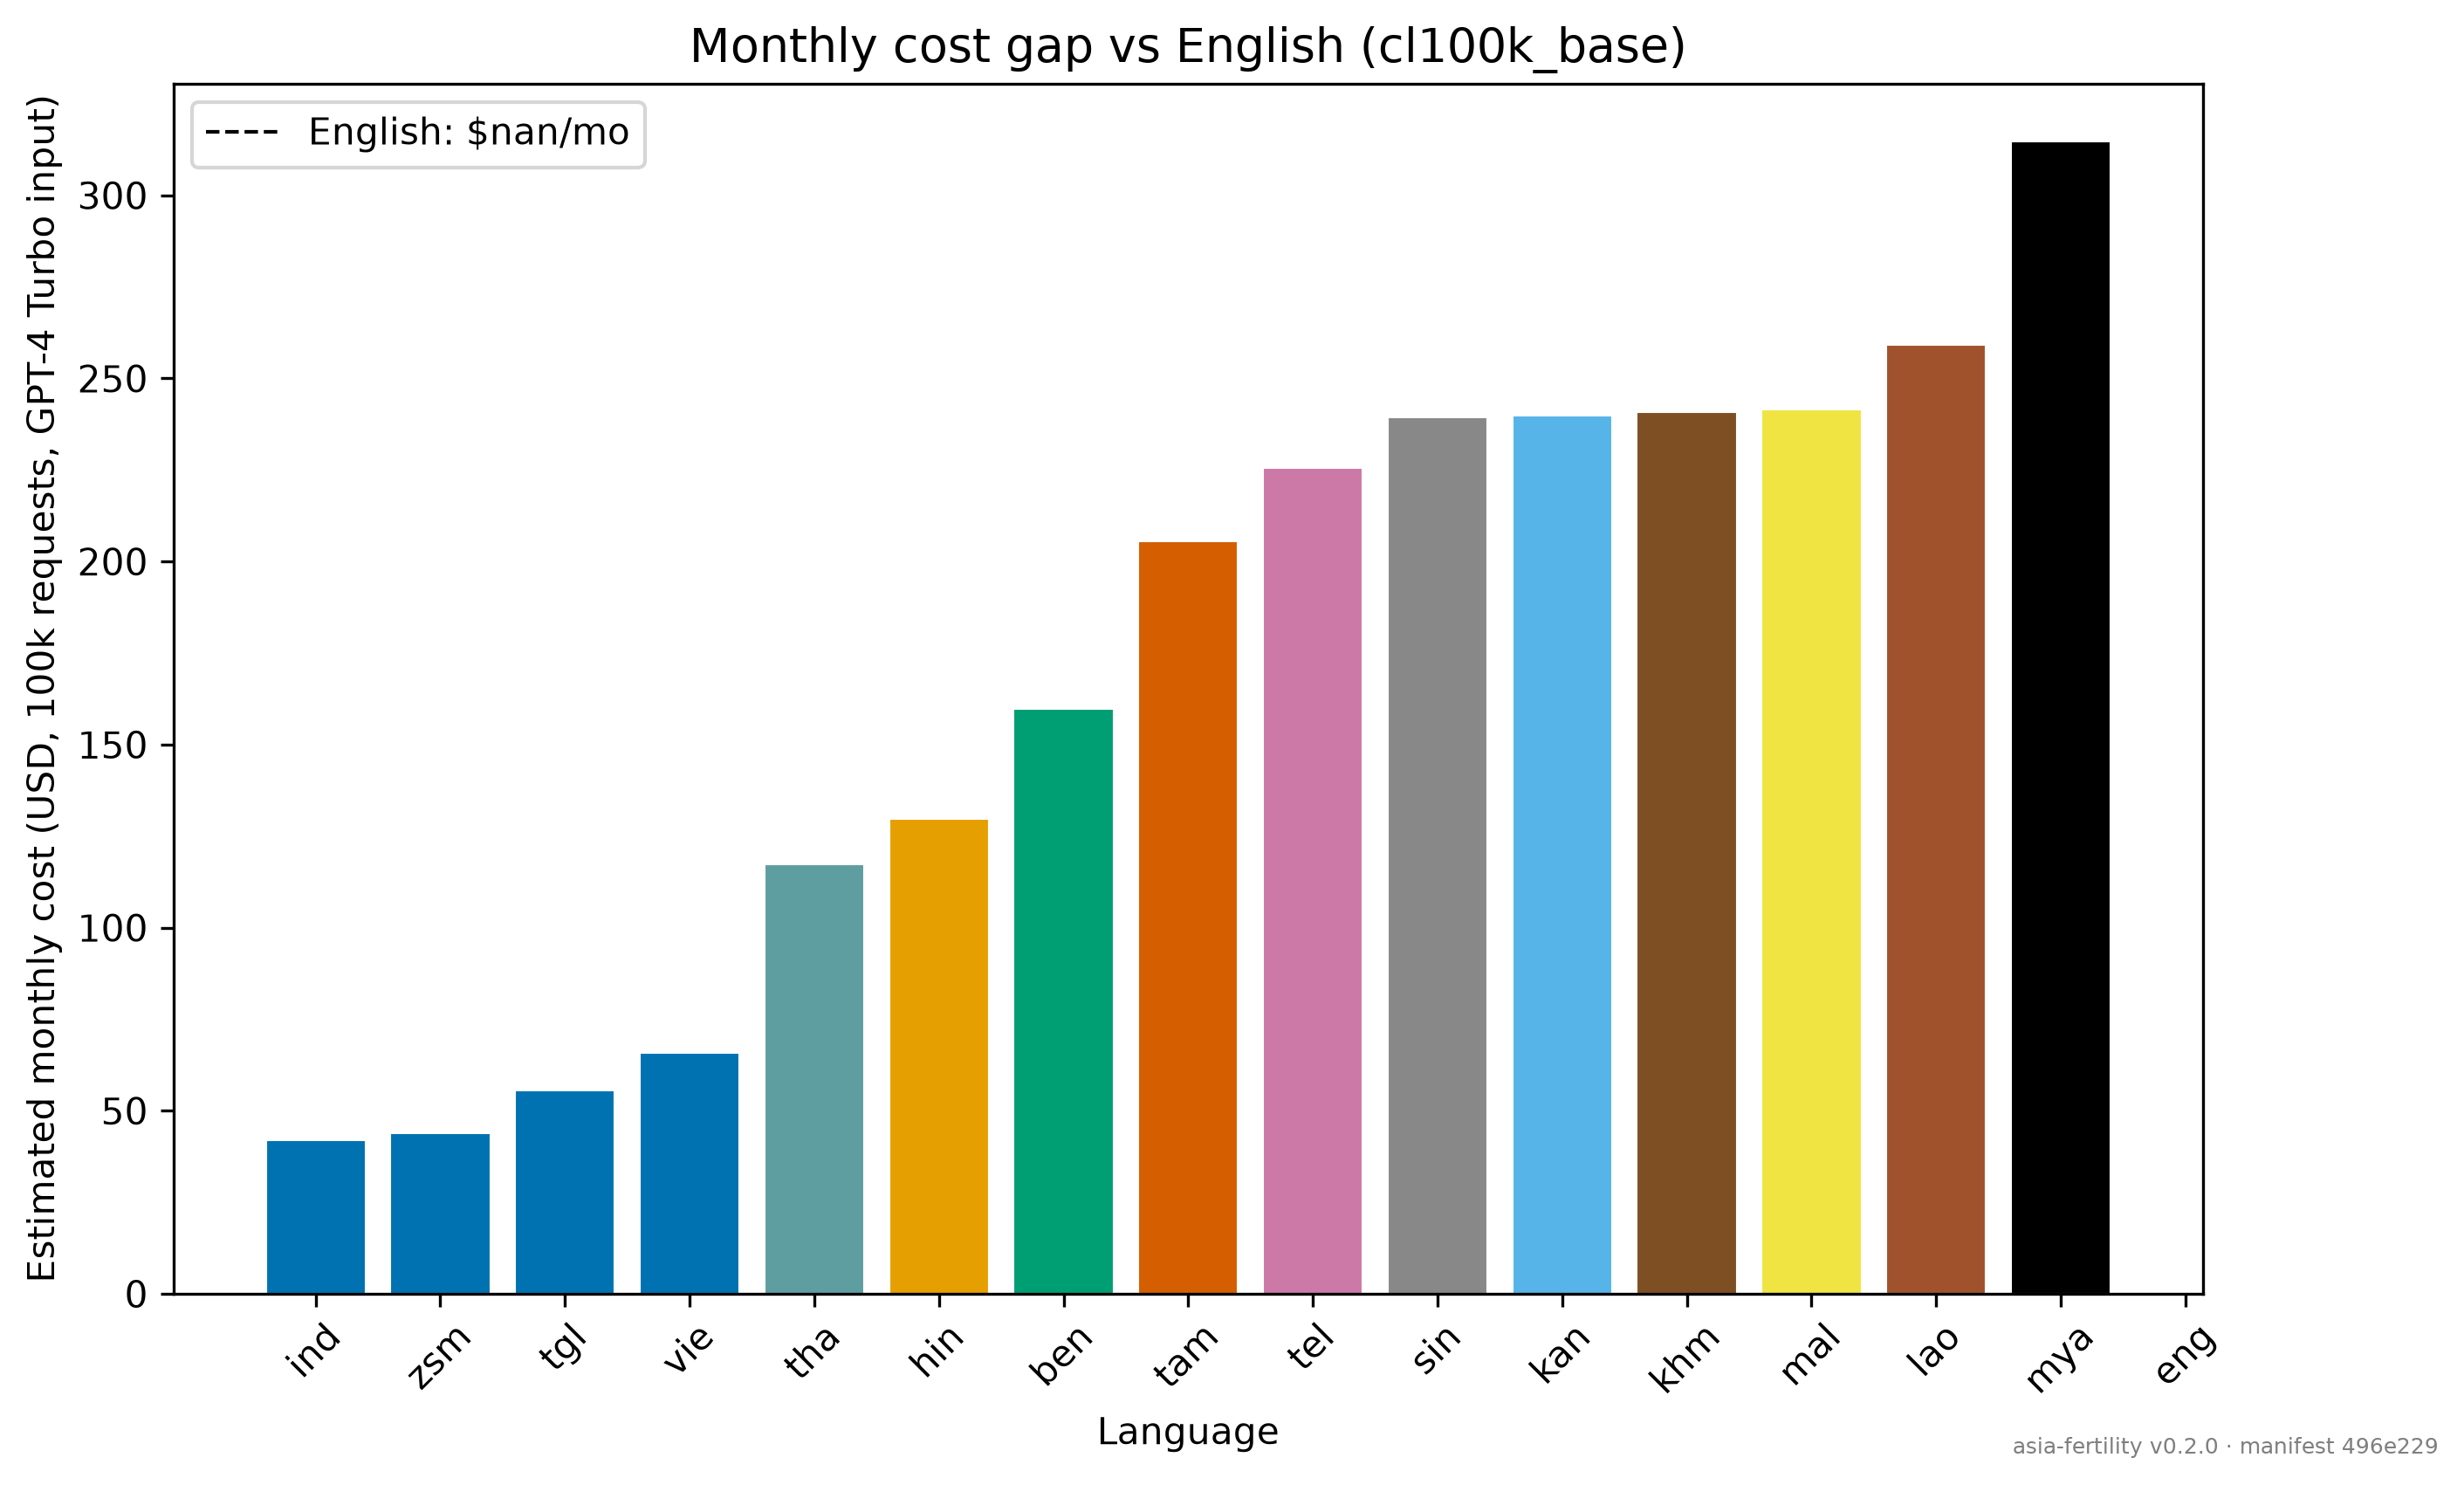
\includegraphics[width=0.85\textwidth]{fig3_cost.png}
\caption{Estimated monthly cost in USD at 100{,}000 requests/month, GPT-4 Turbo input pricing, by language. English baseline marked with the dashed line.}
\label{fig:cost}
\end{figure}

\subsection{Context window exhaustion and in-context capacity}

Figure~\ref{fig:exhaustion} plots cumulative tokens across turns at 100 words/turn. A Burmese or Lao conversation crosses the 4k window in 2--3 turns; the same English conversation lasts ~32 turns. Figure~\ref{fig:capacity} shows the in-context capacity: an 8k-token window holds about 60 hundred-word English examples but only 5--7 for Brahmic-derived scripts.

\begin{figure}[h]
\centering
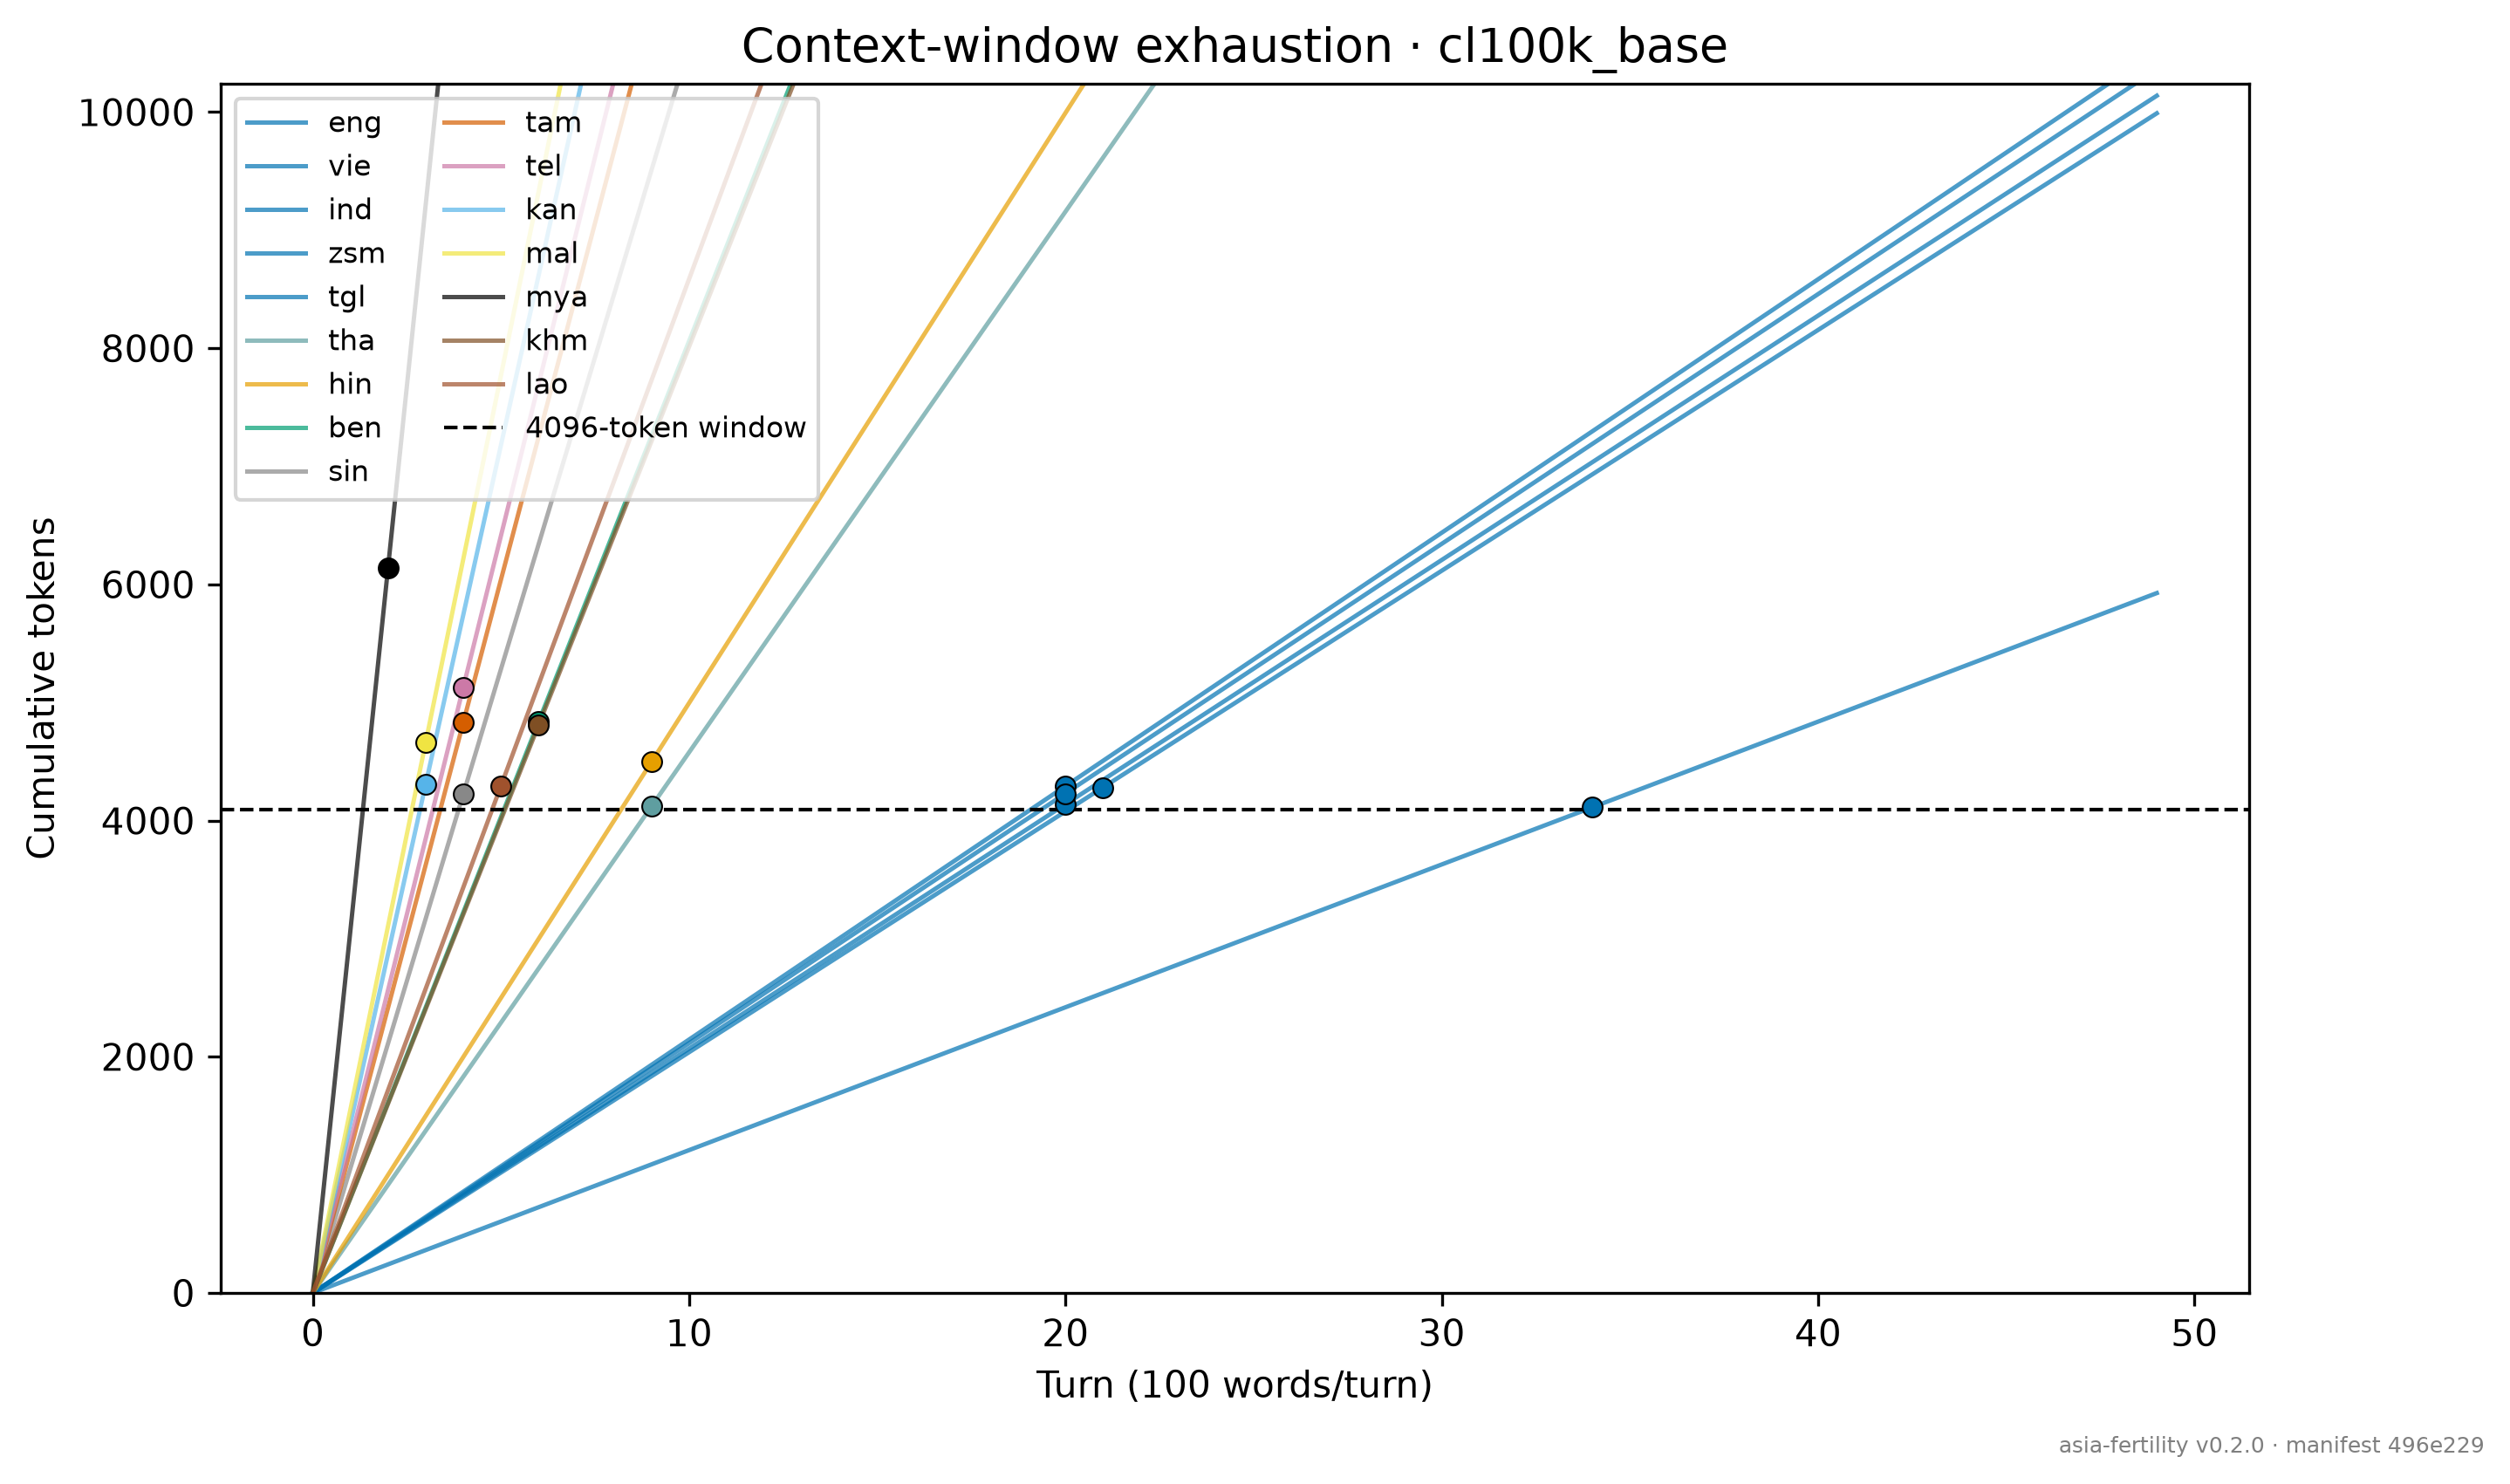
\includegraphics[width=0.85\textwidth]{fig4_context_exhaustion.png}
\caption{Cumulative context use across turns (100 words/turn) on cl100k\_base. Dots mark where each language crosses the 4096-token window.}
\label{fig:exhaustion}
\end{figure}

\begin{figure}[h]
\centering
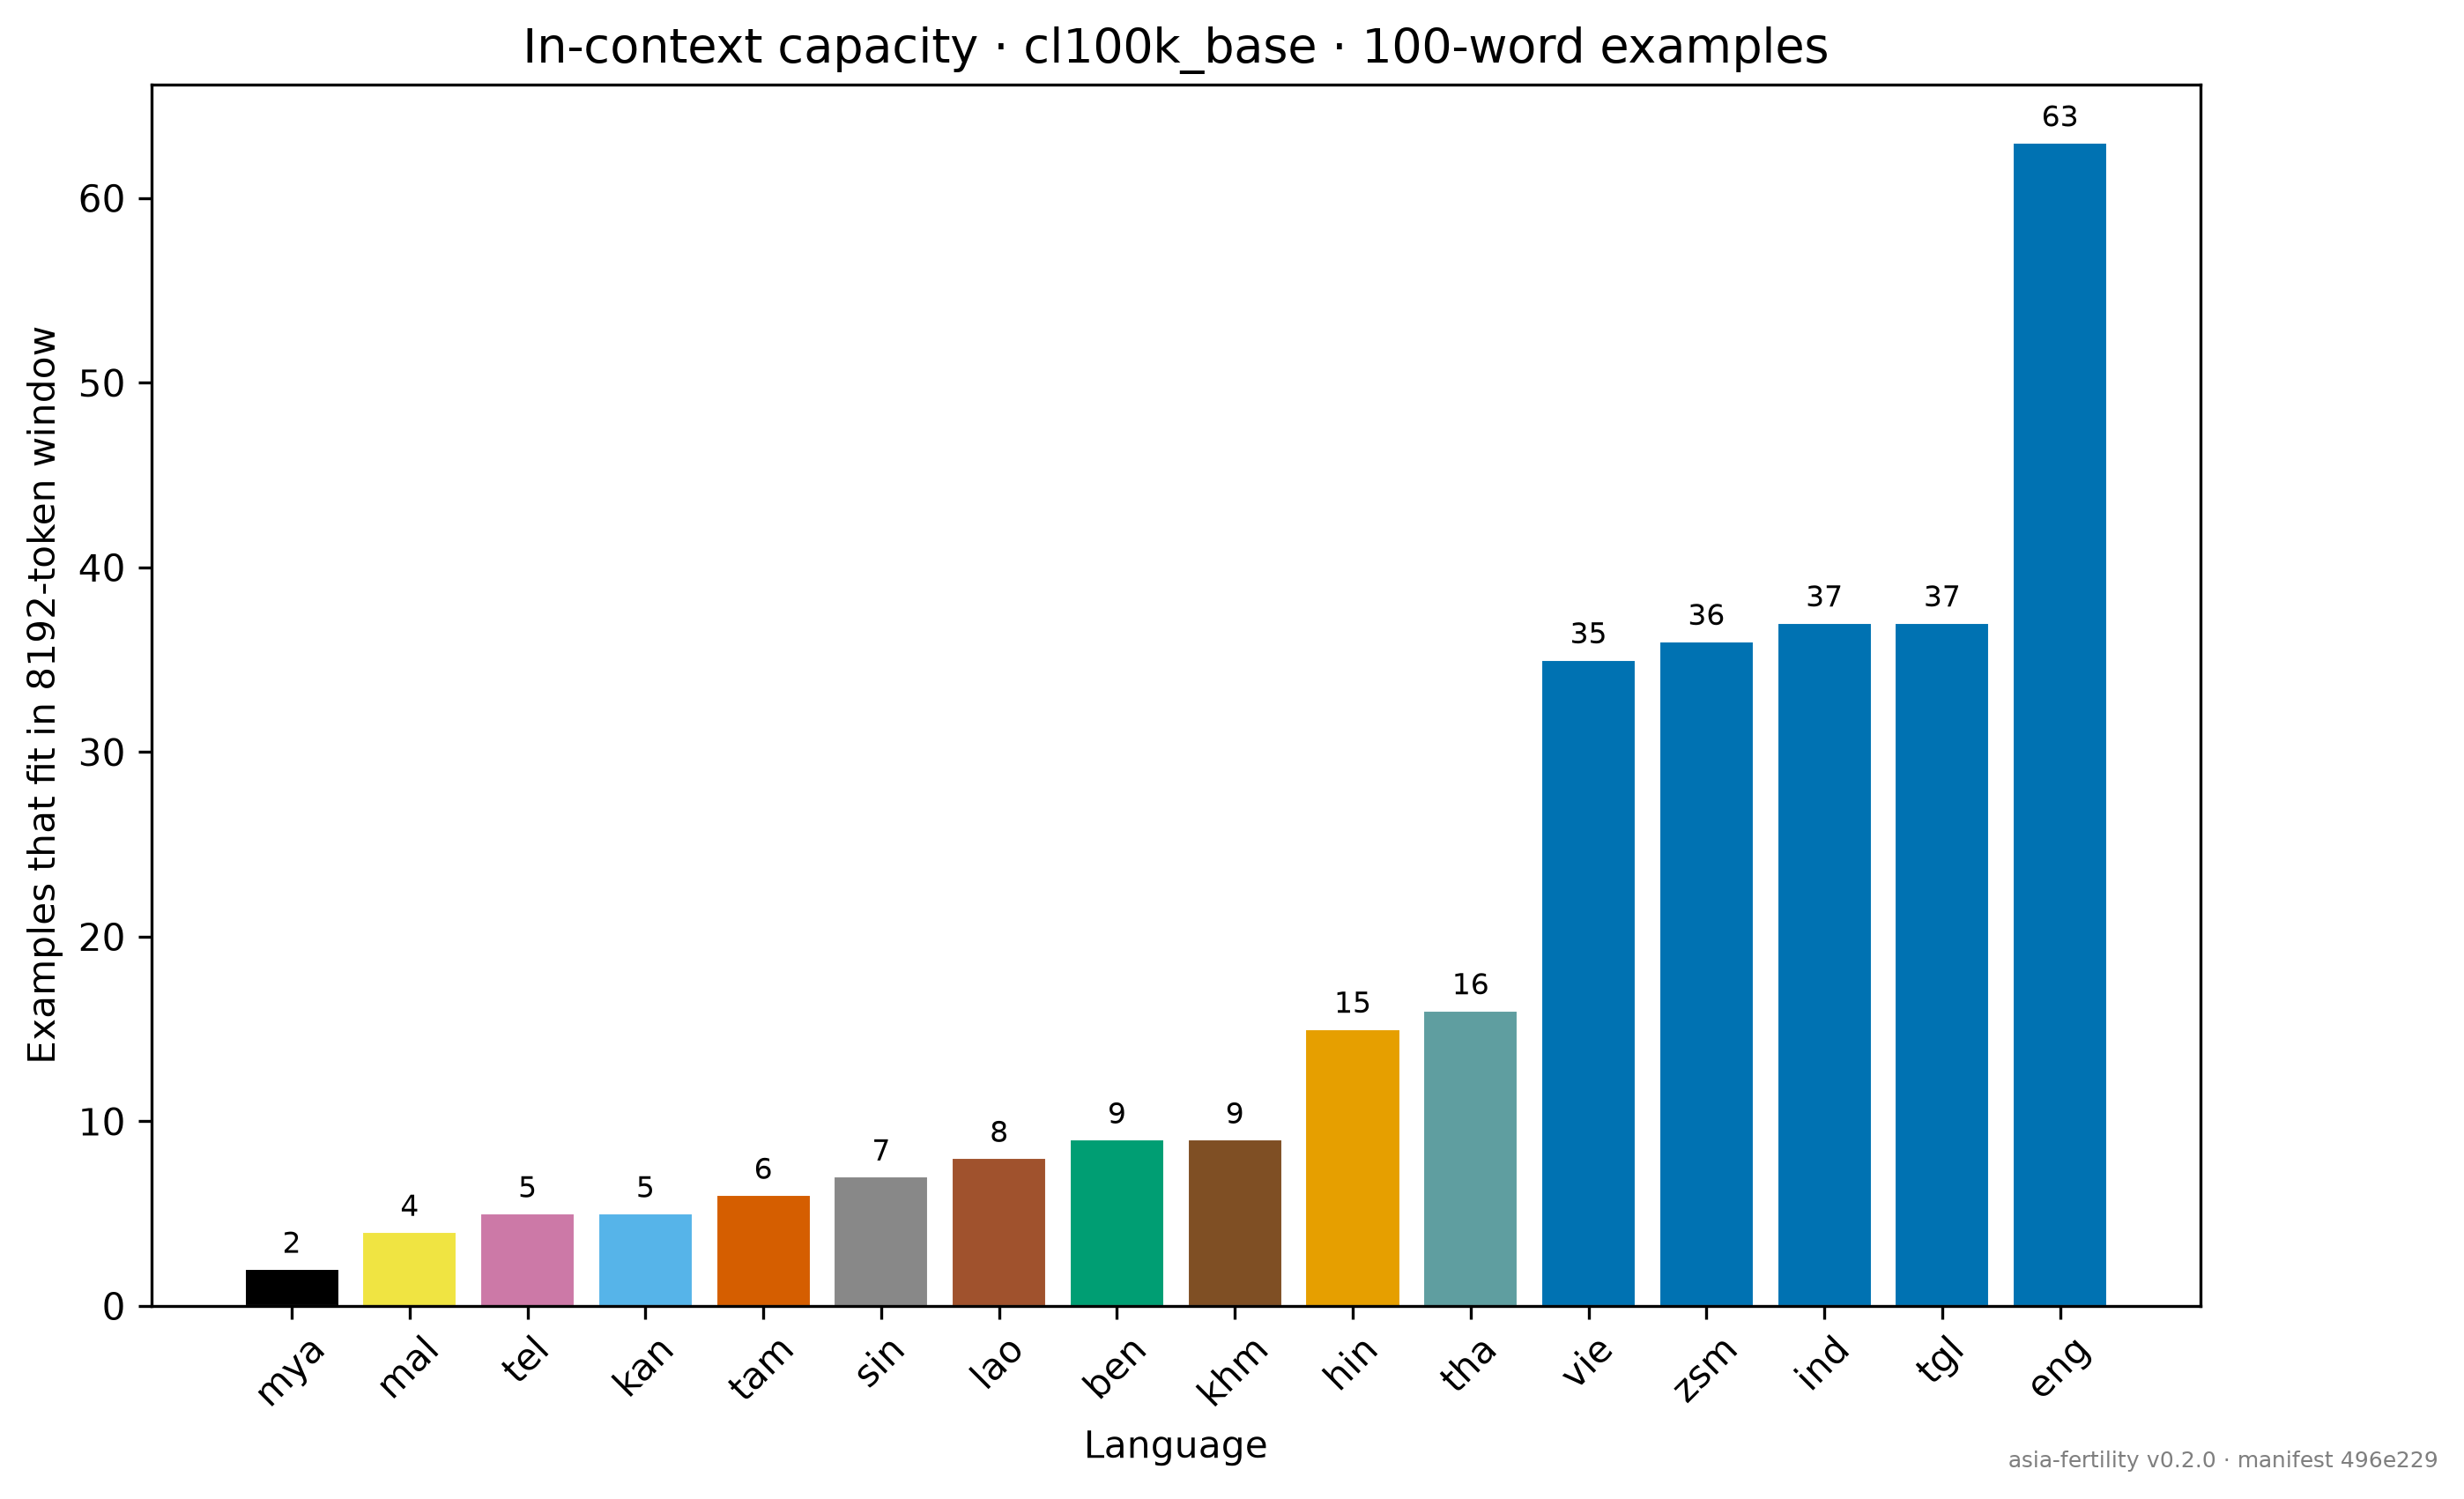
\includegraphics[width=0.85\textwidth]{fig5_in_context_capacity.png}
\caption{Number of 100-word in-context examples that fit in an 8192-token window (cl100k\_base). High-cost languages fit roughly an order of magnitude fewer.}
\label{fig:capacity}
\end{figure}

\subsection{Multi-turn needle-in-haystack recall: a dramatic script-native collapse---except on one model}
\label{sec:recall-results}

We expand the v0.2 pilot's 536-call NIAH benchmark to a \textbf{4\,000-cell} run covering 16 languages $\times$ 5 models $\times$ 5 fill levels (4k, 16k, 32k, 64k, 131k) $\times$ 5 marker positions (5/25/50/75/95\%) $\times$ 2 trials, all via OpenRouter on \texttt{gpt-4o-mini}, \texttt{llama-3.1-8b-instruct}, \texttt{gemini-2.5-flash}, \texttt{qwen-2.5-7b-instruct}, and \texttt{deepseek-chat-v3-0324}. Overall recall pooled across the 4\,000 cells is 36.2\%; the per-model breakdown is presented in Table~\ref{tab:recall-overall} and reveals a sharp separation between one frontier multilingual model and the rest.

\begin{table}[h]
\centering
\small
\begin{tabular}{lrr}
\toprule
Model & Overall recall (16 langs $\times$ 5 fills) & Errors \\
\midrule
\textbf{google/gemini-2.5-flash}          & \textbf{676 / 800 (84.5\%)} & 0 \\
deepseek/deepseek-chat-v3-0324            & 291 / 800 (36.4\%)         & 140 \\
openai/gpt-4o-mini                        & 201 / 800 (25.1\%)         & 230 \\
meta-llama/llama-3.1-8b-instruct          & 160 / 800 (20.0\%)         & 290 \\
qwen/qwen-2.5-7b-instruct                 & 118 / 800 (14.8\%)         & 570 \\
\bottomrule
\end{tabular}
\caption{Overall NIAH recall pooled over 16 languages $\times$ 5 fill levels $\times$ 5 positions $\times$ 2 trials per model. Errors are provider-side failures (context-window overflow). \texttt{gemini-2.5-flash} attains 84\% pooled recall vs.\ 15--36\% for the other four models.}
\label{tab:recall-overall}
\end{table}

Three findings emerge from the per-(model, language) breakdown shown as a recall heatmap in Figure~\ref{fig:recall-heatmap}.

\paragraph{Finding 1: The collapse threshold is 4k, not 64k.} For \texttt{gpt-4o-mini}, \texttt{llama-3.1-8b-instruct}, \texttt{qwen-2.5-7b-instruct}, and \texttt{deepseek-chat-v3-0324}, recall on the 5 Latin-script languages (English, Vietnamese, Indonesian, Malay, Filipino) is 10/10 at the smallest fill level we tested (4\,096 tokens), while recall on the 11 non-Latin Asian languages is 0--2/10 at the same fill. The collapse is therefore \emph{not} depth-driven: it is present already at the smallest context window we measure, and the recall-vs-depth curve for these languages is a flat line at zero. This is a stronger version of the v0.2 finding: the collapse is not concentrated near the model's window edge---it is a property of script-native fragmentation that exists at every depth.

\paragraph{Finding 2: \texttt{gemini-2.5-flash} breaks the pattern.} Across all 16 languages and all 5 fill levels, \texttt{gemini-2.5-flash} attains 76--96\% recall per (model, fill) bucket. Of the 55 non-Latin (lang, fill) cells (11 non-Latin languages $\times$ 5 fills), 38 cells land at 8--10/10 and the worst-case cell---Bengali at 32k---scores 2/10; the median non-Latin cell recall is 8/10, including Burmese at 7--8/10 across most fills and 7/10 specifically at 131k (Figure~\ref{fig:recall-heatmap}). The pooled recall-vs-depth curve is non-monotonic: best at 4k (153/160 = 96\%) \emph{and} at 131k (148/160 = 93\%), with a mild dip at intermediate fills (76--81\%). The other four models, by contrast, collapse to 0--5\% on non-Latin scripts at every fill, and the few non-zero cells they produce are isolated artefacts rather than a coherent recall signal. The collapse is therefore not a fundamental limit of the NIAH task on low-resource scripts: at least one production model retains 84.5\% pooled recall on the same 4\,000-cell grid, which means the failure observed on the other four models is a vendor-level training/serving choice rather than an intrinsic capability boundary.

\paragraph{Finding 3: ``Effective context window'' is language-dependent.} \texttt{deepseek-chat-v3-0324} recalls cleanly at 131k tokens on Latin-script languages (eng/ind/zsm/tgl all at 8--10/10) but errors with HTTP 400 on 100\% of non-Latin haystacks at 131k (110 of 160 cells errored). The cause is not the model's nominal 128k context window: it is that haystacks sized to 131k tokens by the \texttt{o200k\_base} sizing tokenizer expand to 600k+ tokens in DeepSeek's native BPE for high-fertility Brahmic scripts, overflowing the window before inference. Reciprocally, OpenRouter's \texttt{qwen-2.5-7b-instruct} errors at 16k despite a nominal 32k window, and \texttt{llama-3.1-8b-instruct} errors at 32k despite a nominal 128k window---two cases of provider-side effective windows that are shorter than the published model card. \emph{The advertised context window is a property of (model, content language, serving stack) jointly}, and not of the model alone, with the divergence being largest exactly for the languages most expensive to tokenize.

Figure~\ref{fig:recall-heatmap} shows the per-(model, language) recall heatmap with the three findings visible at a glance. Figure~\ref{fig:recall} plots cost ratio vs.\ pooled recall in a per-model panel layout that makes the \texttt{gemini-2.5-flash} outlier the visual centerpiece.

\begin{figure}[h]
\centering
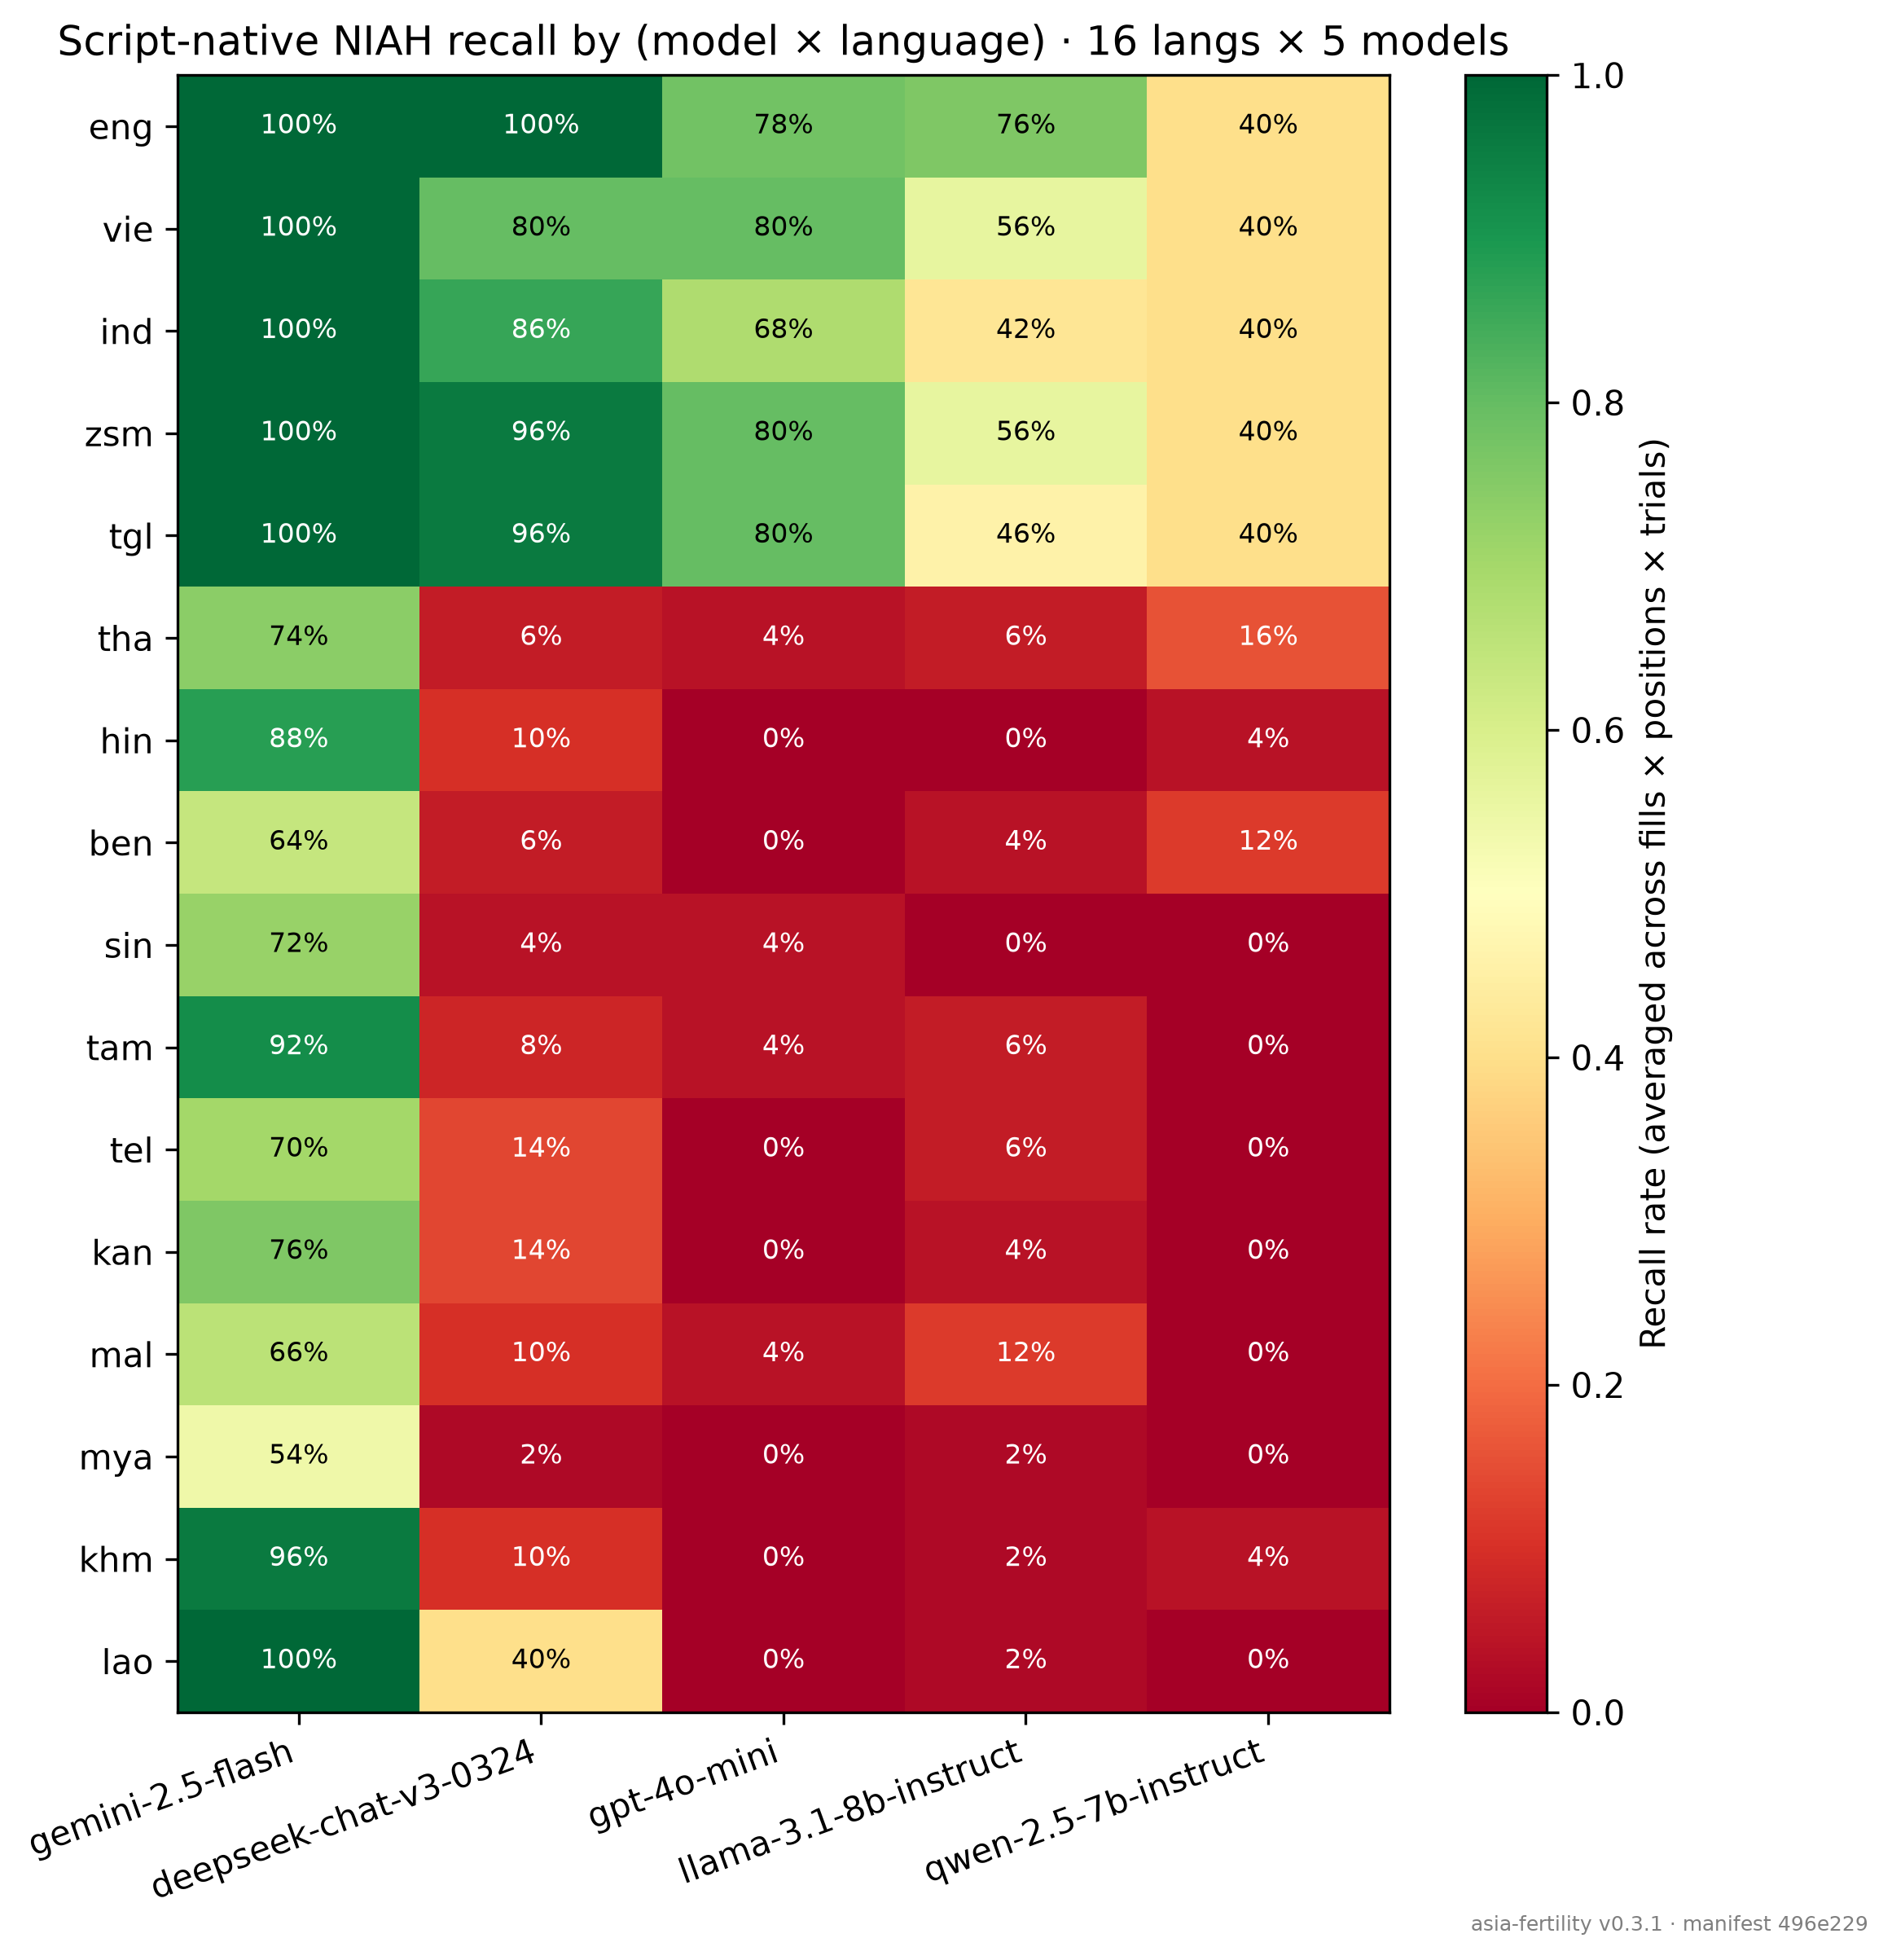
\includegraphics[width=0.95\textwidth]{fig6b_recall_heatmap.png}
\caption{Per-(model, language) NIAH recall heatmap averaged over 5 fill levels $\times$ 5 marker positions $\times$ 2 trials per cell (50 trials per cell). Languages are ordered with Latin scripts at the top. \texttt{gemini-2.5-flash} retains 70--100\% recall across all 16 languages including Brahmic scripts and Burmese; the four other models collapse to 0--20\% on the bottom 11 (non-Latin) rows.}
\label{fig:recall-heatmap}
\end{figure}

\begin{figure}[h]
\centering
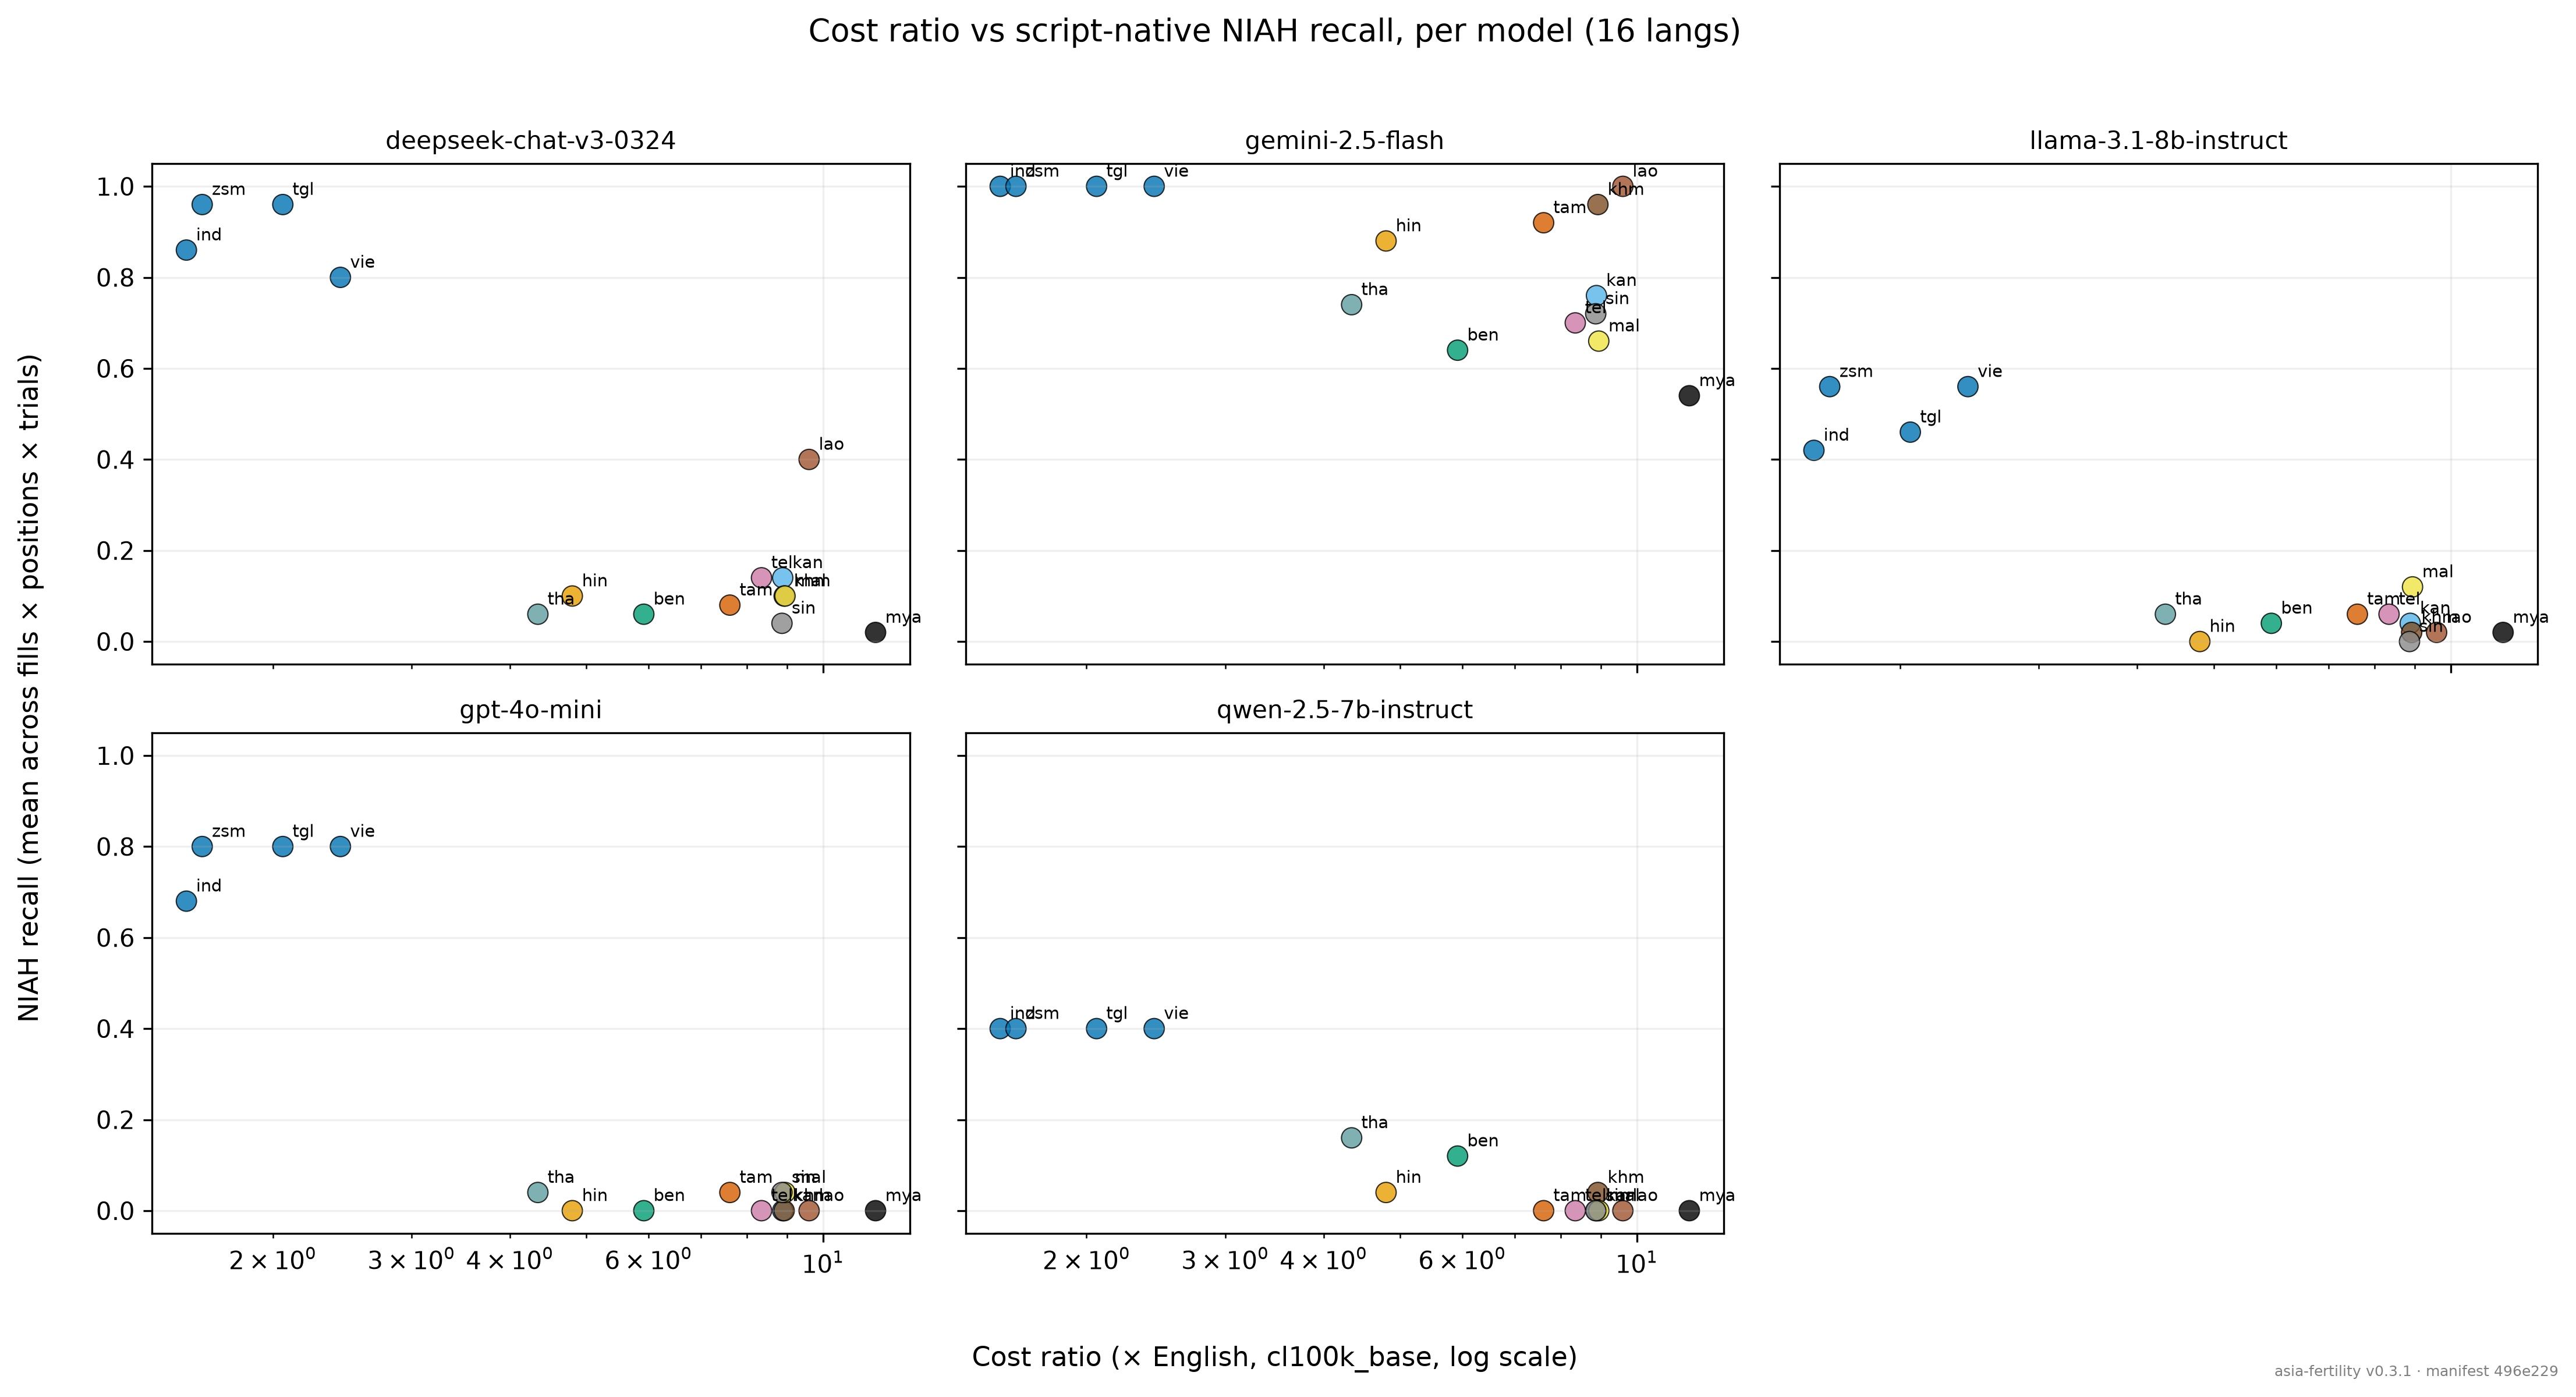
\includegraphics[width=0.95\textwidth]{fig6_premium_vs_recall.png}
\caption{Per-model scatter of cost ratio (\texttt{cl100k\_base}, log scale) vs.\ pooled NIAH recall for each of the 16 study languages, one panel per model. The cost penalty is upstream of any model effect (same x-axis in every panel); the recall response differs by an order of magnitude across vendors. Only \texttt{gemini-2.5-flash} (top-left panel) clears the 70\% recall threshold on the highest-cost languages.}
\label{fig:recall}
\end{figure}

\paragraph{Caveats.} (i) Recall measures the model's ability to retrieve an embedded marker phrase exactly, not its ability to reason over the haystack; \texttt{gemini-2.5-flash}'s advantage is in retrieval and need not extend to comprehension. (ii) Each per-(model, lang, fill, position) cell has $n=2$ trials, so individual cells carry wide confidence intervals; pooled buckets of 10--160 trials are more reliable. (iii) Provider-side serving variance partially confounds the model-vs-vendor distinction: the \texttt{qwen-2.5-7b-instruct} 16k cliff is partly a measurement of OpenRouter's serving infrastructure, not the model. We list these caveats in \S\ref{sec:limitations}.

\subsection{Latency penalty: cost is not a reliable UX proxy}
\label{sec:latency-results}

We additionally measure the \emph{wall-clock latency penalty}: the ratio of measured response time in the target language to English, on the same model. Each (model, language) cell consists of 3 warmup calls (discarded) and 10 timed trials, with each prompt drawn from a distinct FLORES sentence to defeat provider-side prefix caching. Total: 800 measured trials (5 models on OpenRouter---\texttt{gpt-4o-mini}, \texttt{llama-3.1-8b-instruct}, \texttt{gemini-2.5-flash}, \texttt{qwen-2.5-7b-instruct}, \texttt{deepseek-chat-v3-0324}---$\times$ 16 languages $\times$ 10 trials) plus 240 warmup calls (3 per cell), for 1\,040 total HTTP calls. Streaming is enabled to measure both time-to-first-token (TTFT) and total wall-clock time per call.

If \citet{somide2026african}'s finding generalized, we would expect Pearson $r \approx 0.94$ between cost ratio and latency ratio. Instead we observe $r = 0.314$ when pooled across all 5 models, with substantial per-model variance:

\begin{table}[h]
\centering
\small
\begin{tabular}{lc}
\toprule
Model & Pearson $r$ (cost vs.\ latency) \\
\midrule
meta-llama/llama-3.1-8b-instruct & $+0.737$ \\
google/gemini-2.5-flash          & $+0.521$ \\
openai/gpt-4o-mini               & $+0.432$ \\
deepseek/deepseek-chat-v3-0324   & $+0.054$ \\
qwen/qwen-2.5-7b-instruct        & $-0.194$ \\
\bottomrule
\end{tabular}
\caption{Per-model Pearson correlation between same-content cost ratio (cl100k\_base) and measured latency ratio vs.\ English. The relationship is not a property of the language: Llama-3.1's serving stack tracks input fertility linearly ($r = 0.74$), while DeepSeek's and Qwen's do not.}
\label{tab:latency-corr}
\end{table}

\begin{figure}[h]
\centering
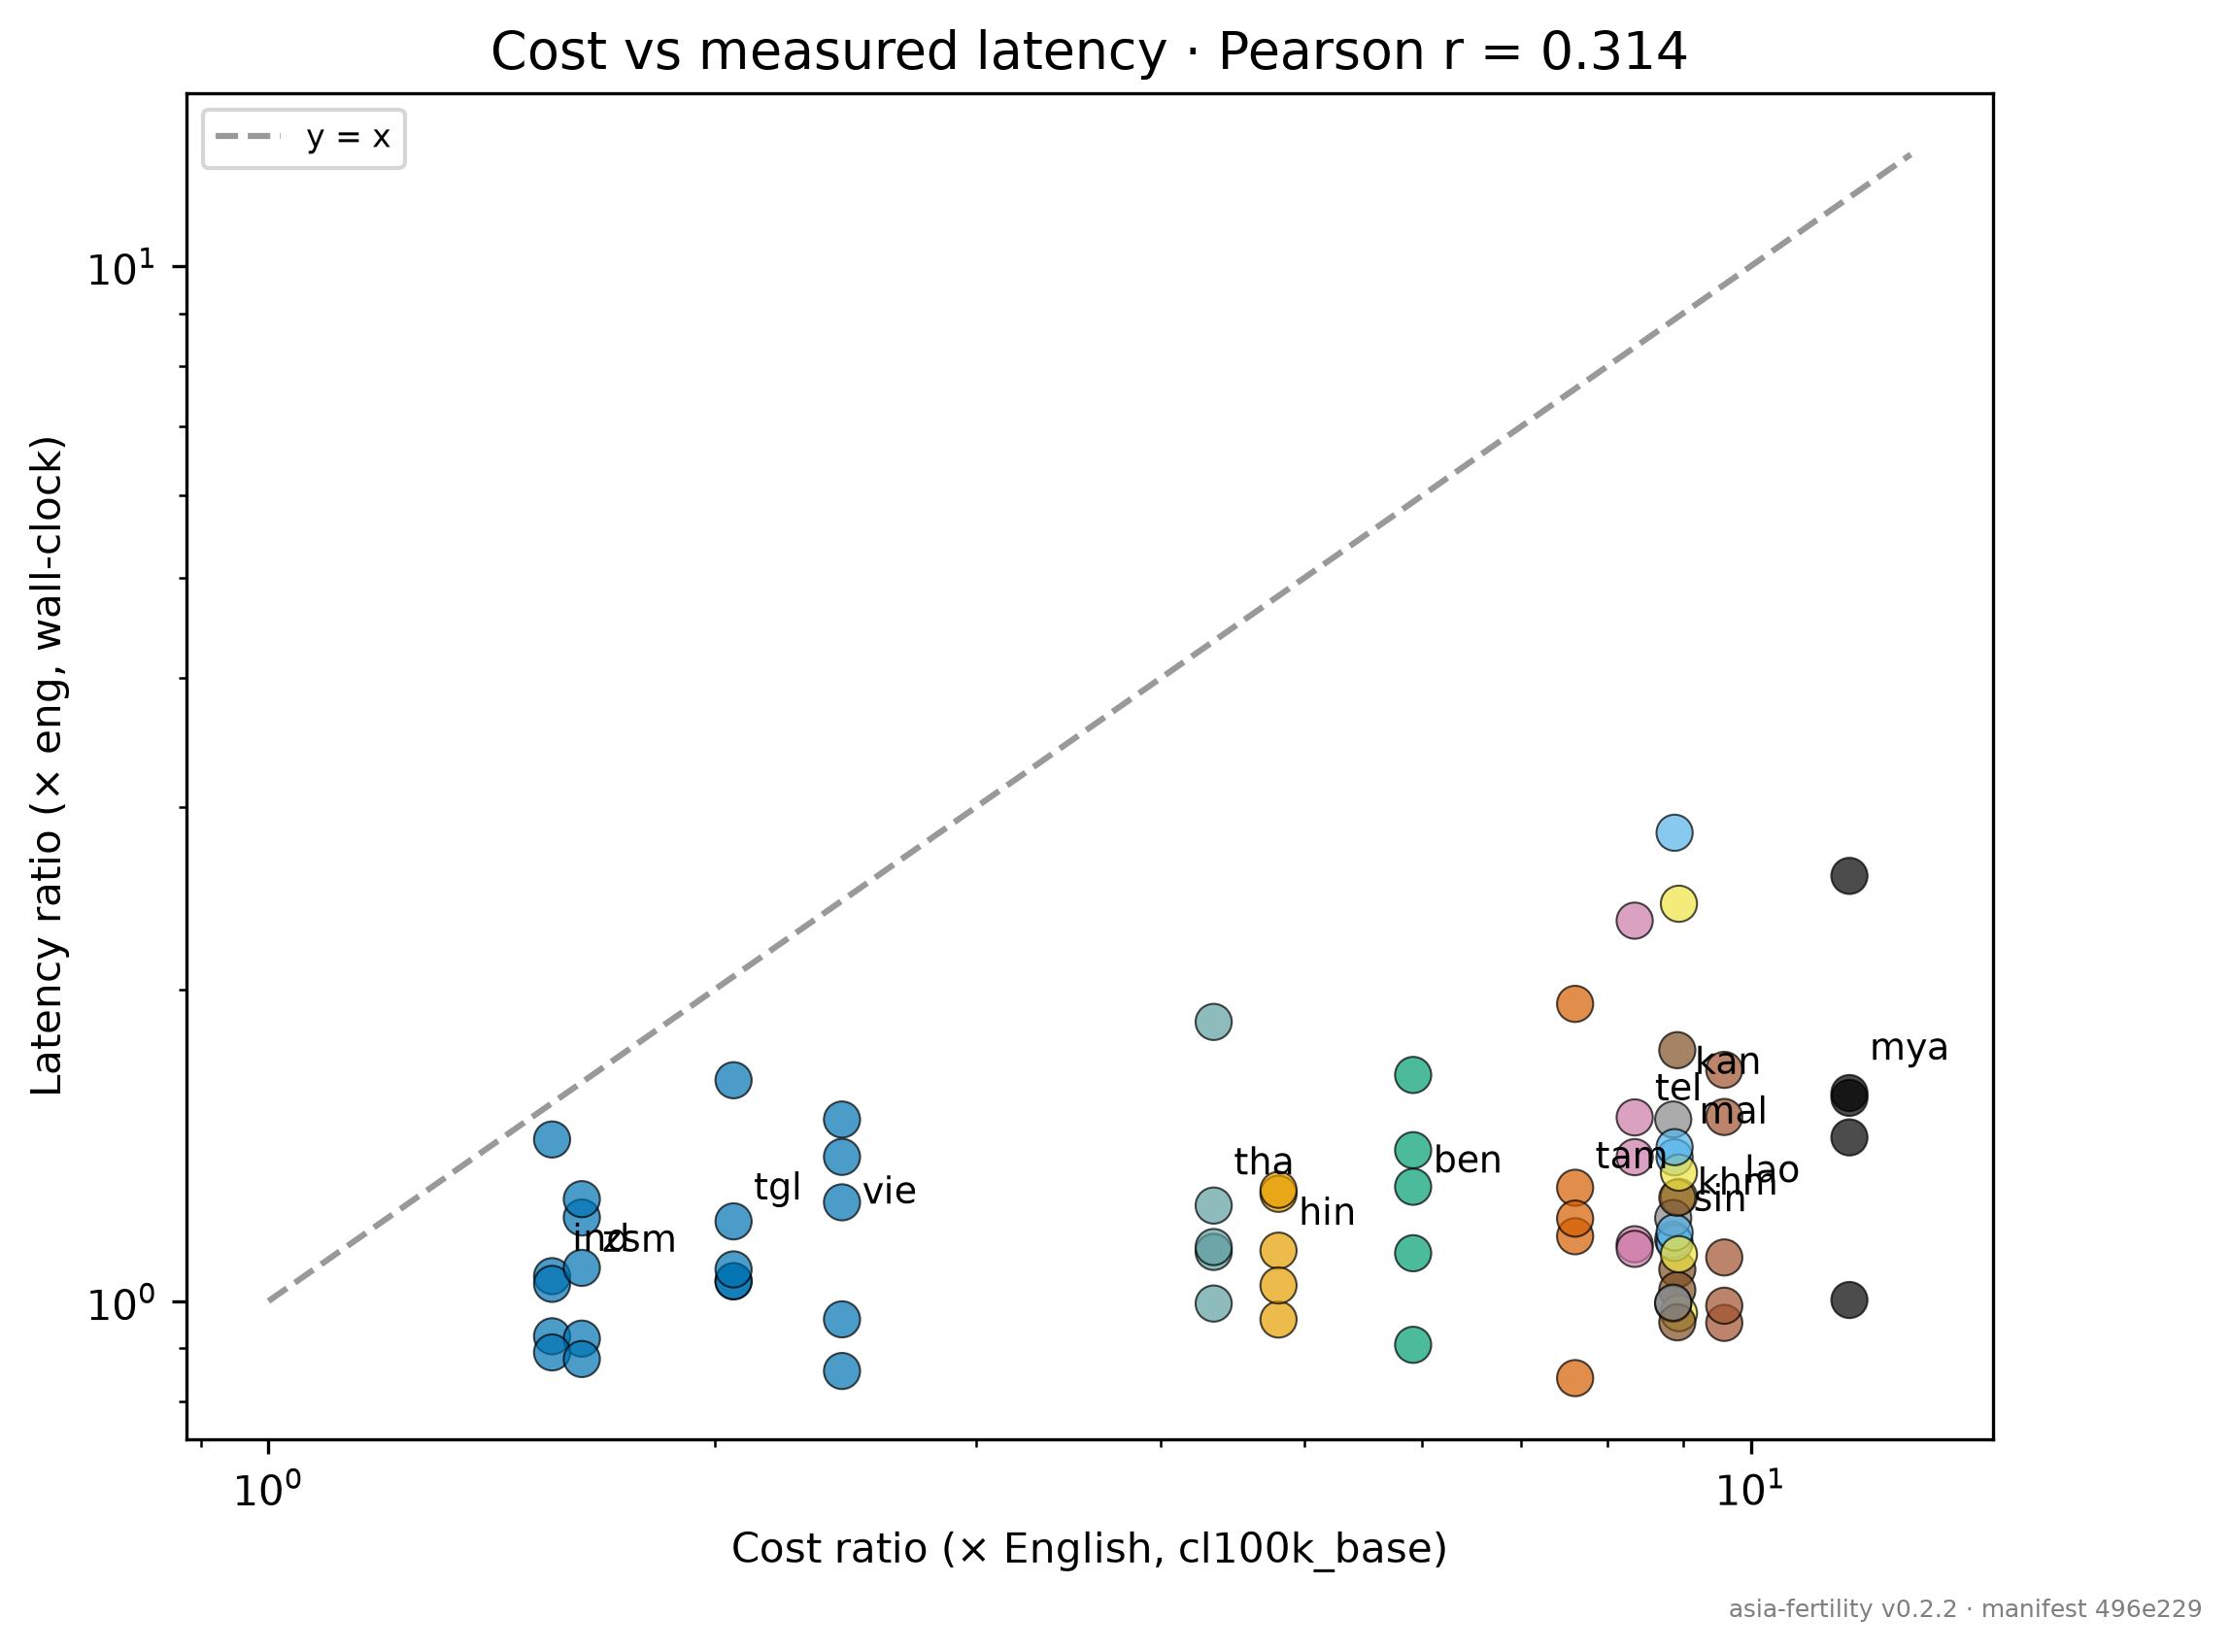
\includegraphics[width=0.85\textwidth]{fig7_cost_vs_latency.png}
\caption{Cost ratio vs.\ measured wall-clock latency ratio per (model, language) cell. Dashed line is $y = x$. Pooled Pearson $r = 0.314$. The cost penalty is upstream of any inference effect; the latency penalty depends on the provider's serving stack (continuous batching, prefill parallelism, dynamic routing). For Burmese on cl100k\_base, the cost ratio is $11.66\times$ while the latency ratio averages only $1.65\times$ across our 5 models---a CFO sees 11$\times$ pain while a user sees roughly 1.5$\times$.}
\label{fig:latency}
\end{figure}

This finding has two consequences. First, \textbf{cost ratio cannot be used as a substitute for latency penalty when reasoning about user experience}: a deployer cannot infer one from the other within a factor of 5. Second, the latency-cost gap appears to be a property of the provider's inference stack rather than of the language itself. Modern continuous-batching and prefill-parallel serving (visible in DeepSeek's and Gemini-Flash's near-flat latency curves) absorbs most of the input-side fertility penalty before it reaches wall-clock time. Llama-3.1-8b, served on older infrastructure, still shows the linear relationship that \citet{somide2026african} reported for their 11-model mix.

\section{Discussion}
\label{sec:discussion}

The tokenizer cost reframes the deployment economics for Asian-language LLM products from ``the model is hard for our language'' (an immutable property) into ``the tokenizer was chosen for English'' (a procurement choice). For Tamil, switching from a cl100k\_base model to an o200k\_base model cuts the bill 3.8$\times$ and the context budget 3.8$\times$, with no model retraining. For Burmese, the analogous switch is 3.7$\times$. For Lao, the picture is bleaker: even the best o200k\_base tokenizer leaves a 8.3$\times$ penalty---no current Western tokenizer covers Lao well.

The NIAH result in \S\ref{sec:recall-results} is the most consequential finding of this work. The 4\,000-cell benchmark shows that on four of five frontier OpenRouter models, recall of script-native markers in non-Latin haystacks collapses to near zero \emph{at all tested fill levels including 4k well inside every model's window}---confirming the v0.2 pilot's collapse finding and extending it across 16 languages, 5 fill levels including 131k, and 5 vendors. Two original-pilot readings remain available. First: the marker is sufficiently fragmented at the subword level that even an attentive model cannot recover it as an exact substring---a \emph{tokenizer-induced representation loss} reading. Second: models cannot attend to script-native subword markers as ``markers'' because their training corpus contains far more Latin marker-like strings than Brahmic ones---a \emph{training-distribution gap} reading. The v0.3 result adds a third reading: \texttt{gemini-2.5-flash}'s 84.5\% pooled recall on the same grid demonstrates that the collapse is not intrinsic to the NIAH task on low-resource scripts, but is a vendor-level choice---most plausibly the presence vs.\ absence of multilingual long-context post-training that includes Brahmic-script data. The three readings are not mutually exclusive; they imply different mitigations (better tokenizers, better pretraining data, better post-training).

The discovery that ``effective context window'' is language-dependent (\S\ref{sec:recall-results}, Finding 3) also has direct implications: capacity-planning systems that assume a model's nominal context window applies to all content languages will silently overflow for high-fertility scripts, exactly the cases where users are already paying the most per character. The asymmetry compounds the cost gap with an availability gap.

\textbf{Comparison to afri-fertility.} Our methodology mirrors \citet{somide2026african}'s methodology: parallel-corpus measurement, sum-then-divide aggregation, pinned price+FX snapshots, manifest-based reproducibility. The two studies are complementary: same penalty, two continents.

\section{Limitations}
\label{sec:limitations}

\textbf{Tokenizer coverage.} The present revision measures 10 tokenizers fully---including \texttt{meta/llama-3.1}, which was ungated by Meta during the period covered by this work and is therefore equivalent to SEA-LION v3's tokenizer for cost-ratio purposes. Specialized Indic tokenizers remain an unfinished extension: at the time of writing, \texttt{sarvamai/sarvam-1} is publicly available and would likely improve Indic numbers further, while the previously-mentioned ``IndicSuperTokenizer'' has no public release under that name (we recommend the AI4Bharat \texttt{IndicBART} family as the closest available substitute for a future v0.4 study). Adding these tokenizers does not change the cost-ratio ordering for the 10 already covered; it would only narrow the absolute Brahmic-script premium reported for cl100k\_base.

\textbf{Domain dependence.} FLORES-200 is news/wiki text. Domain-specific tokenization (medical, legal, conversational) may differ. The \texttt{asia-fertility} package supports user-supplied JSONL/CSV corpora for in-domain measurement.

\textbf{Burmese segmentation.} No widely-installable Burmese word segmentation library exists in 2026; we use a Unicode-block regex syllable segmenter, which inflates word counts relative to ``true'' linguistic words. This affects \emph{fertility} and \emph{premium} (denominator includes words), not the headline \emph{same-content cost ratio} or BPT.

\textbf{NIAH scope.} The 4\,000-cell v0.3 protocol covers 4k--131k tokens but not the 256k--1M window-edge regime that frontier long-context models advertise. \texttt{gemini-2.5-flash}'s non-monotonic recall (best at 4k and 131k, dip in between) hints at position-bias or training-coverage interactions we cannot disentangle without a $\geq$256k extension. Two trials per (model, lang, fill, position) cell also caps the per-cell confidence; bucket-level confidence (10--160 trials) is tighter.

\textbf{Single-author study.} Results reflect one researcher's choices of tokenizers, marker design, and metric definitions; cross-replication encouraged.

\section{Conclusion}
\label{sec:conclusion}

We measured the multilingual tokenizer tax across 16 Asian languages and 10 tokenizers (including \texttt{meta/llama-3.1}, now ungated), with 95\% bootstrap confidence intervals on the full FLORES-200 dev split. The penalty is real, large (up to 11.7$\times$ on cl100k\_base for Burmese), tokenizer-dependent (3--6$\times$ reduction with a byte-level vocabulary), and visible before any model is invoked. Our 4\,000-cell NIAH benchmark with script-native markers shows that the cost penalty is compounded by a \emph{recall} penalty on four of five frontier OpenRouter models, present already at 4k tokens, and that ``effective context window'' is language-dependent. Crucially, \texttt{gemini-2.5-flash} attains 84.5\% pooled recall on the same 4\,000-cell grid where the other four models score 15--36\%, demonstrating that the script-native collapse is a vendor-level training choice and not a fundamental limit of the task.

The cost penalty is a procurement choice, not a property of language difficulty. Our open-source \texttt{asia-fertility} package lets any team verify the tax on their own text before they choose a model.

\section*{Code and Data Availability}
\begin{itemize}
    \item Package: \url{https://github.com/Helmo21/asia-fertility} (MIT). \texttt{pip install asia-fertility[oai]; asia-fertility reproduce}.
    \item HuggingFace dataset: \url{https://huggingface.co/datasets/Helmo21/asia-fertility} (CC-BY-SA 4.0).
    \item Manifest with SHA256 of config, pinned price + FX snapshots, and tokenizer versions accompanies each run.
\end{itemize}

\section*{Acknowledgements}
This work builds on the FertiScope hackathon submission at the Global South AI Safety Hackathon, Da Nang, June 2026, with Leo Dang, Miles Whiticker, and Vinh Van as co-authors of the original paper. The present arXiv-style writeup expands on that work with bootstrap CIs, the BPT metric, a wider tokenizer set, full FLORES-200 dev rather than a 50-sentence subset, an 800-trial wall-clock latency benchmark (plus 240 warmup calls), and a 4\,000-cell NIAH benchmark with script-native markers across five frontier OpenRouter models and 16 languages. The methodological framing closely follows \citet{somide2026african}'s African Language Tax paper, with which the present work forms a complementary pair.

\bibliographystyle{plainnat}
\bibliography{refs}

\end{document}
